\chapter{ACE-Transfer Integrals} \label{ch:4}

In this chapter, we present an alternative approach for predicting transfer integrals (electronic couplings) of organic molecular dimers using \textsc{ACEpotentials.jl}. Instead of employing standard atomic neighbour representations, we introduce two alternative schemes, namely, \textit{Bead} (\textit{Coarse-Grained}) and \textit{Heavy-atom} representations.

This methodology is motivated by the physical origin of transfer integrals, which are determined by atomic and molecular orbital couplings.
It is therefore reasonable to group the transfer integrals associated with individual atomic orbitals into effective molecular orbitals of a coarse-grained system or to focus specifically on molecular orbitals localised on carbon atoms (e.g., C–H coupling orbitals).

We outline how to build ACE descriptors that are customised to handle various input datasets and  analyse which representations are well suited for different classes of molecular dimers.

Section~\ref{sec:4.1} highlights the significance of transfer integrals in organic semiconductors.
We then discuss the symmetries of the transfer integrals and how we incorporate them into ACE models in section~\ref{sec:4.11}.
Section~\ref{sec:4.2} provides an analysis of the naphthalene dimer's transfer integral energy surfaces.
The transfer integrals of its uniform configurations are calculated from the quantum chemistry package \textsc{PyMOO}, ZINDO-based method~\cite{Kirkpatrick2007}.
%ring-structured molecular dimers, specifically naphthalene and thiophene dimers. 
It also covers the construction of ACE descriptors within the \textit{Bead} and \textit{Heavy-atom} frameworks, along with the fitting results and discussions that follow.
In Section~\ref{sec:4.3}, we apply the approach to other simpler molecular dimers (ethylene and thiophene). Their rnadom configuration's transfer integrals, generated from \textsc{xtb-dipro} package~\cite{Kohn2023}, are used to train the ACE model. 
We then evaluate the predictive capability of the \textit{Heavy-atom} representations within the ACE framework.
Finally, we conclude with a summary of the main findings and outline potential directions for future work in Section~\ref{sec:4.4}.

\section{Transfer Integrals in Organic Semiconductors} \label{sec:4.1}
\begin{figure*}[t]
\centering

\includegraphics[width=0.75\textwidth]{Figure/Chapter 4/MO.jpg}
\caption{\label{fig:4.1} 
Coupling between frontier molecular orbitals (FMOs) of two conjugated organic molecules. The top and bottom FMOs represent the coupling between the lowest unoccupied molecular orbitals (LUMO–LUMO) and the coupling between the highest occupied molecular orbitals (HOMO–HOMO), respectively.
    }
\end{figure*}

Organic semiconductors are now essential components for lightweight, flexible electronics. 
Charge carriers in organic materials are frequently localised, unlike in inorganic semiconductors, where charge transport occurs through band-like conduction.

The active layer of the organic semiconductors is typically composed of $\pi$-conjugated molecular systems, in which overlapping $\pi$-orbitals allow for the delocalisation of $\pi$-electrons along the molecular backbone. 
This $\pi$-electron delocalisation facilitates the formation of frontier molecular orbitals, shown in Figure~\ref{fig:4.1}, that are critical for transport processes.

Regarding the discussion in section \ref{sec:2.6}, transport processes can be determined by the electronic coupling between two molecular sites and influence the rate of charge hopping transports, defined as the transfer integrals $J$
\[
J_{ab} = \langle \psi_a | \hat{H} | \psi_b \rangle,
\]
where $\psi_a$ and $\psi_b$ denote the frontier molecular orbitals on the respective molecular sites, and $\hat{H}$ is the electronic Hamiltonian.
Practically, we can parameterise $J_{ab}$ using the relative centre-of-mass displacement $(x_{ab}, y_{ab}, z_{ab})$ and the relative rotational orientations $(\theta_x, \theta_y, \theta_z)$ between two molecules, illustrated in Figure~\ref{fig:4.2}.

\begin{figure*}[t]
\centering

\includegraphics[width=0.65\textwidth]{Figure/Chapter 4/Acceptor.jpg}
\caption{\label{fig:4.2} 
Schematic illustration of charge transport in organic semiconductors. The active layer consists of an intermixed donor/acceptor morphology between anode and cathode electrodes. A zoomed-in view shows the electronic coupling between two $\pi$-conjugated molecules (Mol $a$ and Mol $b$), characterised by their relative centre-of-mass displacement $(x_{ab}, y_{ab}, z_{ab})$ and relative rotational orientations $(\theta_x, \theta_y, \theta_z)$. The transfer integral $J_{ab}$, governing the charge transfer rate between molecules, is a function of these relative coordinates.}
\end{figure*}

In Marcus theory, the transfer integrals can be employed to calculate the charge transfer rate $k$ between two molecular sites, given by
\begin{equation} \label{equ:4.1}
    k = \frac{2\pi}{\hbar} |J|^2 \frac{1}{\sqrt{4\pi\lambda k_B T}} \exp\left( -\frac{(\Delta G + \lambda)^2}{4\lambda k_B T} \right),
\end{equation}

where $\lambda$ is the reorganisation energy, $\Delta G$ is the Gibbs free energy change, $k_B$ is Boltzmann’s constant, and $T$ is the temperature.
The rate depends quadratically on the magnitude of the transfer integral $|J|^2$, implying that precise predictions of $J$ are critical for reliable modelling of charge transport phenomena in organic materials.

However, predicting transfer integrals presents several challenges.
\begin{itemize}
    \item Direct quantum chemical calculations are computationally expensive, particularly for large datasets of molecular dimers \cite{Troisi2011}.
    Accurately computing $J$ typically requires electronic structure methods such as density functional theory (DFT) or fragment orbital approaches, which become prohibitively costly when thousands of molecular configurations must be evaluated, or the molecular assembles contain thousands of atoms.
    \item Transfer integrals are highly sensitive to molecular geometry \cite{Troisi2006}; even small structural perturbations can lead to significant variations in $J$.
    Thermal fluctuations, molecular vibrations, and slight changes in intermolecular orientation can all induce large deviations in the electronic coupling, leading to the difficulty of generalising results across different configurations.
    %\item Finally, the development of efficient surrogate models is essential to enable large-scale simulations of charge transport in realistic systems \cite{Fratini2016}.
    %Without fast and accurate predictions of $J$, it is impractical to simulate dynamic processes such as charge diffusion over long timescales or in disordered organic materials.
\end{itemize}

Applying a machine learning potential approach, particularly in frameworks based on the atomic cluster expansion (ACE), offers a promising alternative.
By learning the mapping between molecular configurations and transfer integrals, ACE-based models can achieve high predictive accuracy across diverse geometries while significantly reducing computational costs compared to traditional \textit{ab initio} methods.

\section{ACE Model Incorporation} \label{sec:4.11}

The purpose of this study is to estimate the transfer integrals \( J_{ab} \) between molecules \(a\) and \(b\) utilising the Atomic Cluster Expansion (ACE) model.

We first recast the site enegery in Eq.~\eqref{equ:2.78} for the multi-element system
\begin{equation}
\label{equ:12}
\begin{split}
    \epsilon(\left\{\mathbf{x}_{ij}\right\}_{j\sim i}) =& 
    \sum_{{\bm\zeta}{\bf nlm}}  
    c^{(Z_i)}_{{\bm\zeta}{\bf nlm}} \textbf{B}_{{\bm \zeta}\mathbf{nl}\mu}^{(i)},
%     \sum^{N}_{\nu=0}\;\sum_{\mathbf{nlm}}
% c^{(\nu)}_{\mathbf{nlm}}\textbf{B}^{(\nu)}_{\mathbf{nlm}}(\mathbf{r}_{i{j}_{1}},\cdots,\mathbf{r}_{i{j}_{\nu}}). \\
\end{split}
\end{equation}
Similar to Equation~\eqref{equ:12}, the \textit{site} transfer integral may be articulated by determining the parameter \(\tilde{c}\) as follows: 
\begin{equation} \label{equ:13} 
\ \mathcal{J}_{ab}\left(\{\mathbf{x}_{ij}\}_{j \sim i}\right) 
= \sum_{{\bm\zeta}{\bf nlm}} \tilde{c}^{(Z_i)}_{{\bm\zeta}{\bf nlm},ab} \mathbf{B}^{(i)}_{{\bm \zeta}{\bf nlm}}, 
\end{equation} 
where the chemical species \(Z_i\) and the index \({\bm\zeta}\) need not correspond to actual atomic species but may be designated as a \textit{pseudo-atomic species} (any categorical variable representing an abstract particle), as elaborated in next section.

Upon ascertaining the parameters $\tilde{\bm c}$ for the model in Equation~\eqref{equ:13}, the overall transfer integral of the molecular dimer system is subsequently formulated as a summation of the \textit{site} contributions. 
\begin{equation}
\label{equ:14}
J_{ab}\!\left(\{\mathbf{x}_{i}\}_{i=1}^{J}\right) 
= \sum_{i=1}^{J} 
\mathcal{J}_{ab}\!\left(\{\mathbf{x}_{ij}\}_{j \sim i}\right).
\end{equation}


 Text in bold Symmetry concerns.  
 The transfer integrals \(J_{ab}\) adhere to three essential symmetry constraints dictated by the electronic Hamiltonian: (i) Hermitian symmetry (\(J_{ab}=J_{ba}^*\)), (ii) spatial invariance under rotations and translations, and (iii) localisation of electronic interactions.  
 In developing the ACE model in Equations~\eqref{equ:13} and~\eqref{equ:14}, we expressly guarantee the preservation of all these qualities.

 The transfer integral between molecular orbitals \(\psi_a\) and \(\psi_b\) is defined as 
\[J_{ab} = \langle \psi_a | \hat{H} | \psi_b \rangle,\]
which, due to the Hermiticity of the Hamiltonian \(\hat{H} = \hat{H}^\dagger\), adheres to the following condition: 
 \begin{equation}
\label{equ:15}
J_{ab} = J_{ba}^*.
\end{equation}
 In systems with real-valued molecular orbitals, this simplifies to \(J_{ab} = J_{ba}\), signifying that the transfer integral is a \textit{symmetric scalar quantity} upon the interchange of monomers \(a\) and \(b\).  
 This property is inherently maintained in the ACE representation via symmetric parameterisation of the coefficients \(\tilde{c}^{(Z_i)}_{{\bm\zeta}{\bf nlm},ab}\) or through training on symmetrised data, hence ensuring that 
\begin{equation}
\label{equ:16}
\mathcal{J}_{ab}\!\left(\{\mathbf{x}_{ij}\}_{j \sim i}\right)
= \mathcal{J}_{ba}\!\left(\{\mathbf{x}_{ij}\}_{j \sim i}\right).
\end{equation}

 Given that the transfer integrals are contingent solely upon the relative geometry of the molecular dimer, rather than its absolute position or orientation, the ACE basis functions \(\mathbf{B}^{(i)}_{{\bm\zeta}{\bf nlm}}\) are formulated to exhibit both rotational and translational invariance, thereby ensuring that 
\begin{equation}
\label{equ:17}
J_{ab}\!\left(\{\mathbf{x}_{i}\}_{i=1}^{J}\right)
= J_{ab}\!\left(\{\mathbf{x}_{i}'\}_{i=1}^{J}\right),
\quad \text{for} 
\mathbf{x}_i' = \hat{\mathbf{Q}}\mathbf{x}_i + \mathbf{t},
\end{equation}
 where \(\hat{\mathbf{Q}}\) denotes an arbitrary rotation matrix and \(\mathbf{t}\) represents a translation vector.  
 The ACE framework explicitly encodes these symmetry requirements by constructing descriptors and basis functions that remain invariant under the Euclidean group \(E(3)\), which includes all rotations, translations, and reflections.  
 Consequently, the resultant model parameters \(\tilde{\mathbf{c}}\) inherently ensure rotational and translational invariance without requiring explicit data augmentation.

 The spatial decomposition of the \textbf{single particle basis function} in Equation~\eqref{equ:2.79} illustrates the location of electronic interactions.  
 In quantum mechanics, the total coupling can be expressed as a summation of local orbital-orbital interactions, 
 \begin{equation} 
 \label{equ:18}
 J_{ab} = \sum_{i \in a} \sum_{j \in b} \langle \phi_i | \hat{H} | \phi_j \rangle, 
 \end{equation}
 Because each term diminishes swiftly with increasing interatomic distance due to the localised characteristics of atomic orbitals.  
 Analogously, each site contribution \(\mathcal{J}_{ab}(\{\mathbf{x}_{ij}\})\) in the ACE model relies solely on adjacent atoms within a defined cut-off radius, guaranteeing that \(J_{ab}\) is represented as a summation of local, symmetry-preserving contributions:
\begin{equation} 
\label{equ:19}  
\mathcal{J}_{ab}\!\left(\{\mathbf{x}_{ij}\}_{j \sim i}\right) = \mathcal{J}_{ab}\!\left(\{\mathbf{x}_{ij}\}_{|\mathbf{x}_{ij}| < r_\mathrm{cut}}\right).
\end{equation} 

\section{Naphthalene Dimer} \label{sec:4.2}

This section presents the transfer integral energy surface analysis of the naphthalene dimer. This naphthalene dimer are rigid and fully parameterised with 6 DoF. Moreover, the dimer is relatively small, leading to rapid transfer integral calculations. Therefore, it is sensible to begin modelling their transfer integrals as a starting point.

Two alternative frameworks, the \textit{Coarse-Grained} and \textit{Heavy-atom} representations, are employed to construct ACE descriptors. 
Each representation's predictive performance is assessed by fitting the transfer integrals derived from calculations involving quantum chemistry, and the outcomes are then discussed.

We intend to evaluate the ACE methodology's ability to capture the dependence of electronic couplings on molecular configurations by looking at the naphthalene systems.

\subsubsection{Analysis of Transfer Integral Surface}
We begin by investigating the surfaces of the transfer integrals. 
As discussed in Section~\ref{subsec:2.6.4}, many studies predict transfer integrals based on either the square or the absolute value of the transfer integrals, since these quantities correlate linearly with the charge transfer rate.  
However, the surface of the squared transfer integrals $J^2$ is typically discontinuous and highly skewed, containing many small values and a few large peaks, resulting in non-smooth behaviour that poses challenges for machine learning models based on smooth basis sets.
\begin{figure*}[t]\centering
\begin{subfigure}{.33\textwidth}
  \centering
  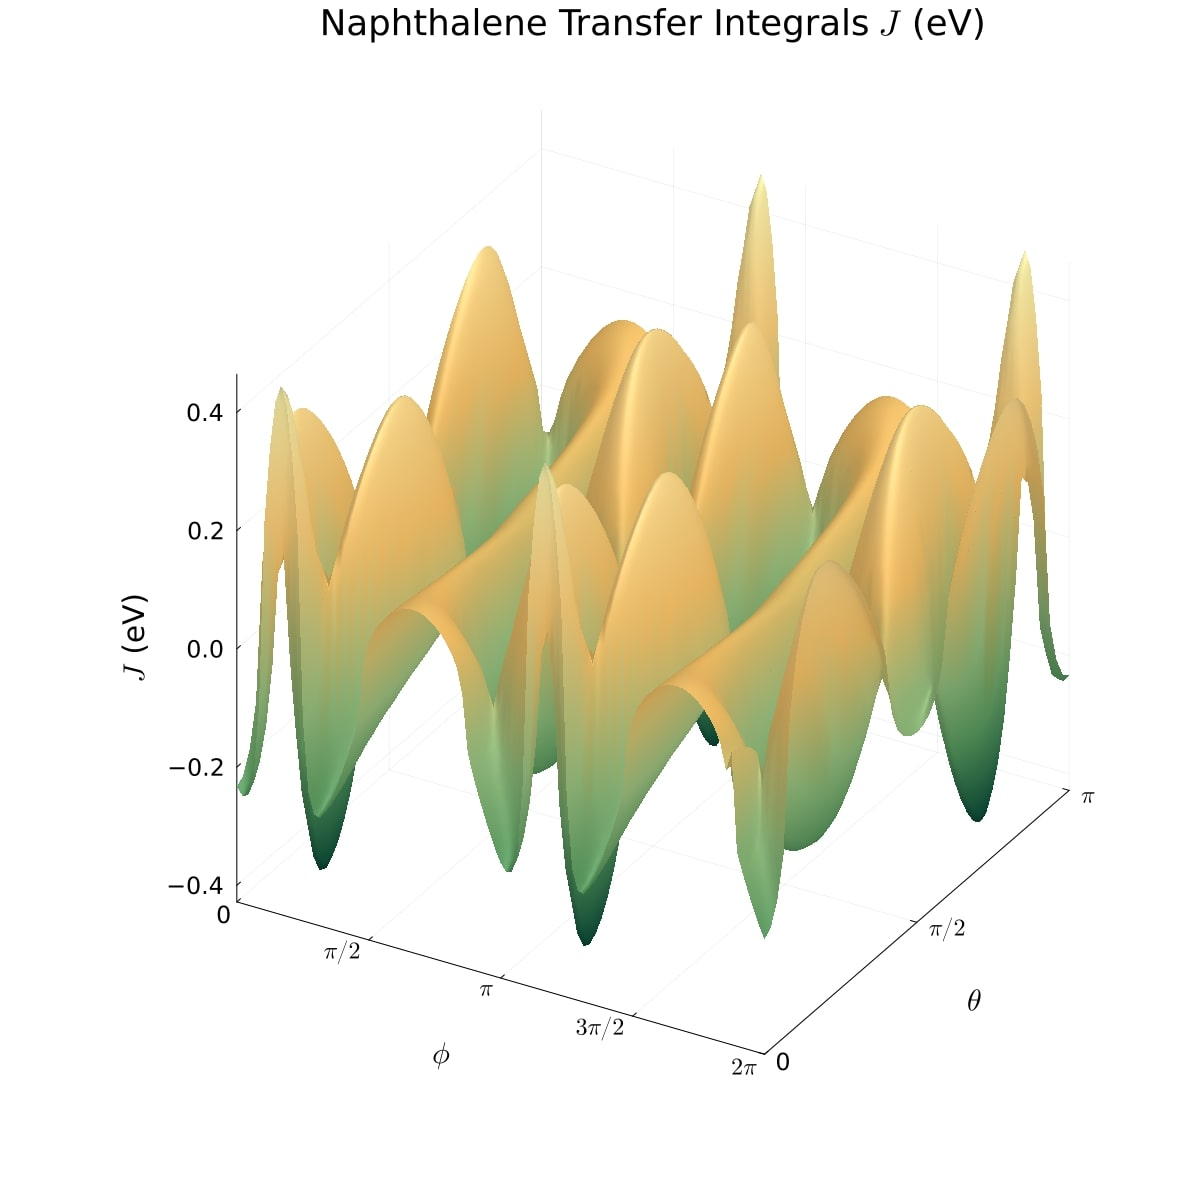
\includegraphics[width=1\linewidth,height=\textheight,keepaspectratio]{Figure/Chapter 4/1_Naphthalene/new_Naphthalene_J_surface.jpg}
  \caption{}
\end{subfigure}%
\begin{subfigure}{.33\textwidth}
  \centering
  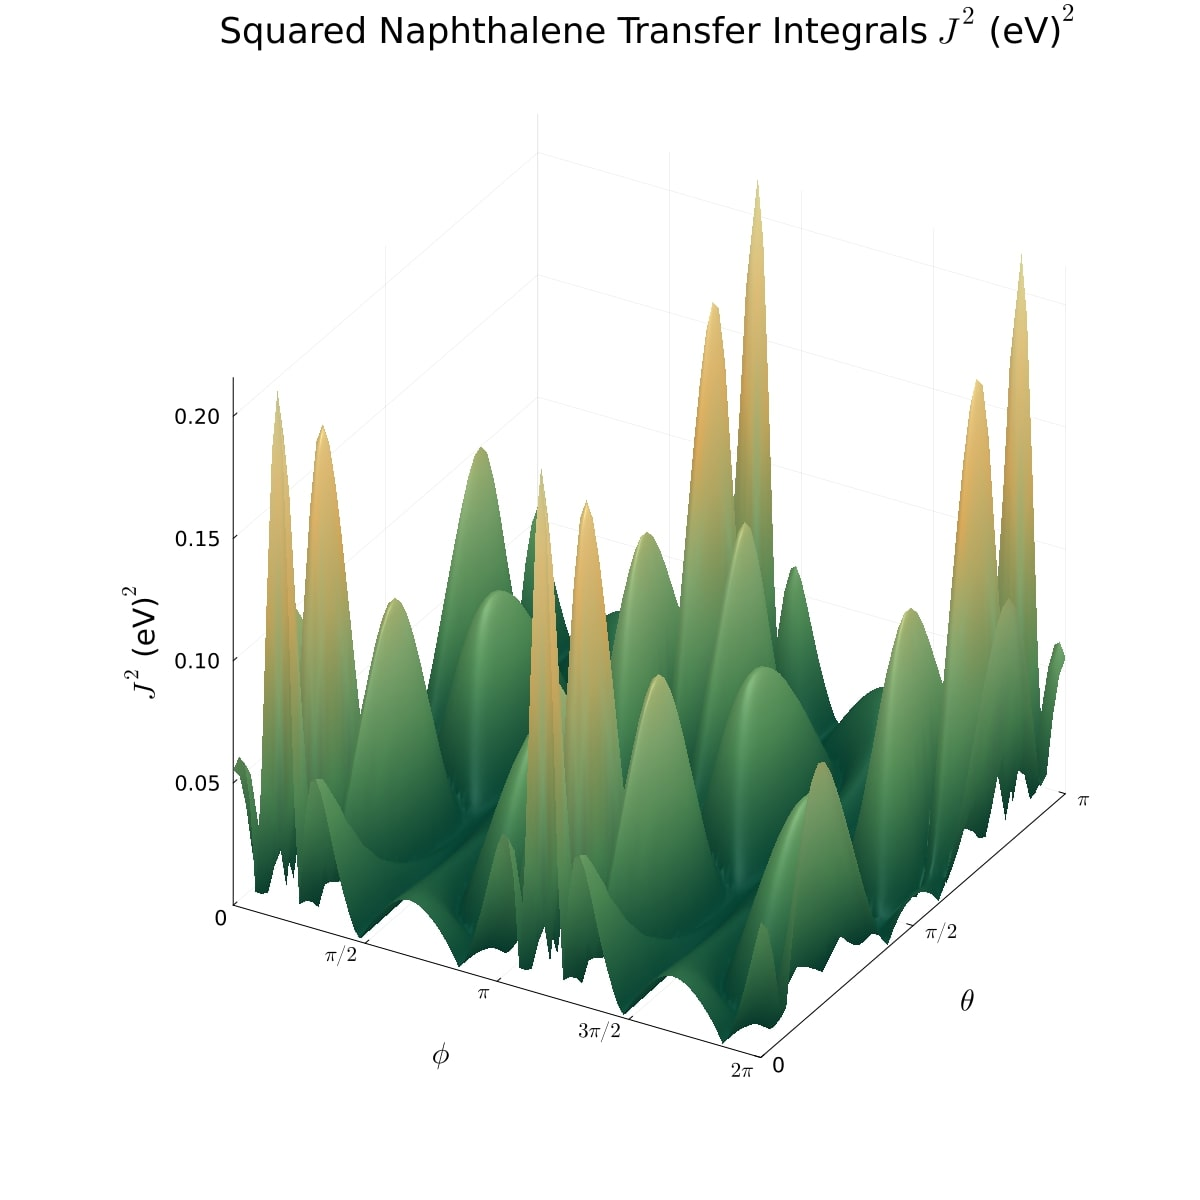
\includegraphics[width=1\linewidth,height=\textheight,keepaspectratio]{Figure/Chapter 4/1_Naphthalene/new_Naphthalene_J^2_surface.jpg}
  \caption{}
\end{subfigure}%
\begin{subfigure}{.33\textwidth}
  \centering
  \includegraphics[width=1\linewidth,height=\textheight,keepaspectratio]{Figure/Chapter 4/1_Naphthalene/new_Naphthalene_logJ^2_surface.jpg}
  \caption{}
\end{subfigure}
\caption{
    \label{fig:4.3}
        (a), (b), and (c) show the surface plots of the transfer integral $J(\theta, \phi)$ of a naphthalene dimer, the squared transfer integral $J^2(\theta, \phi)$, and the logarithm of the squared transfer integral.
}
\end{figure*}

Since ACE models are constructed from a set of smooth basis functions, fitting highly non-smooth quantities such as $J^2$ may be particularly sensitive to the choice of basis parameters. 
In such cases, training models directly on the transfer integrals $J$ or on the logarithm of the squared transfer integrals, $\log(J^2)$, can improve predictive capability. 
Both $J$ and $\log(J^2)$ produce distributions that are smoother and more Gaussian-like, which are well suited for regression tasks.

Figures~\ref{fig:4.3} and~\ref{fig:4.3.1} illustrate the three $2d$-surfaces and heatmaps corresponding to the transfer integral of the naphthalene dimer: the transfer integral itself, its squared value, and the logarithm of its squared value. 
These surfaces are parameterised by the orientational angles $\theta \in [0, \pi]$ and $\phi \in [0, 2\pi]$ of molecule $b$ with respect to molecule $a$, as depicted in Figure~\ref{fig:4.2}. 
In other words, molecule $b$ is rotated over the surface of the sphere around molecule $a$, at a fixed centre-of-mass distance of 12~\AA.
It is evident that the surfaces of the squared transfer integrals (Figure~\ref{fig:4.3}b and~\ref{fig:4.3.1}b) and the logarithm of the squared transfer integrals (Figures~\ref{fig:4.3}c and~\ref{fig:4.3.1}c) exhibit sharp singularities, whereas the transfer integrals $J$ (Figure~\ref{fig:4.3}a and~\ref{fig:4.3.1}a) are smoother by comparison.
This observation suggests that choosing appropriate target quantities, such as $J$, is critical for achieving efficient and accurate ACE model fitting.
\begin{figure*}[t]\centering
\begin{subfigure}{.32\textwidth}
  \centering
  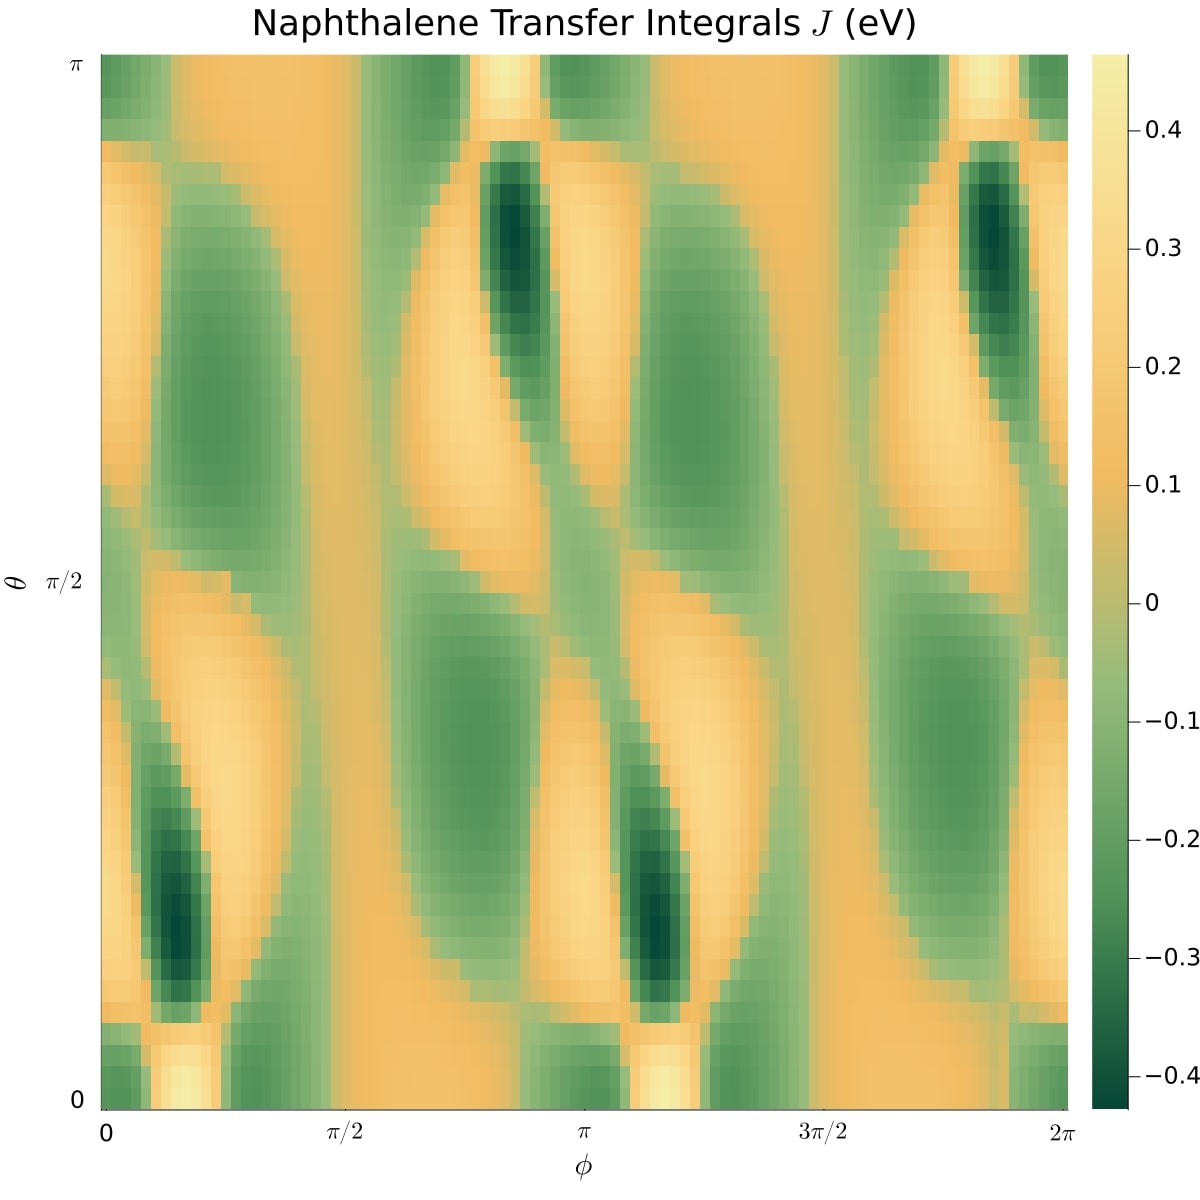
\includegraphics[width=1\linewidth,height=\textheight,keepaspectratio]{Figure/Chapter 4/1_Naphthalene/new_Naphthalene_J_heatmap.jpg}
  \caption{}
\end{subfigure}
\begin{subfigure}{.32\textwidth}
  \centering
  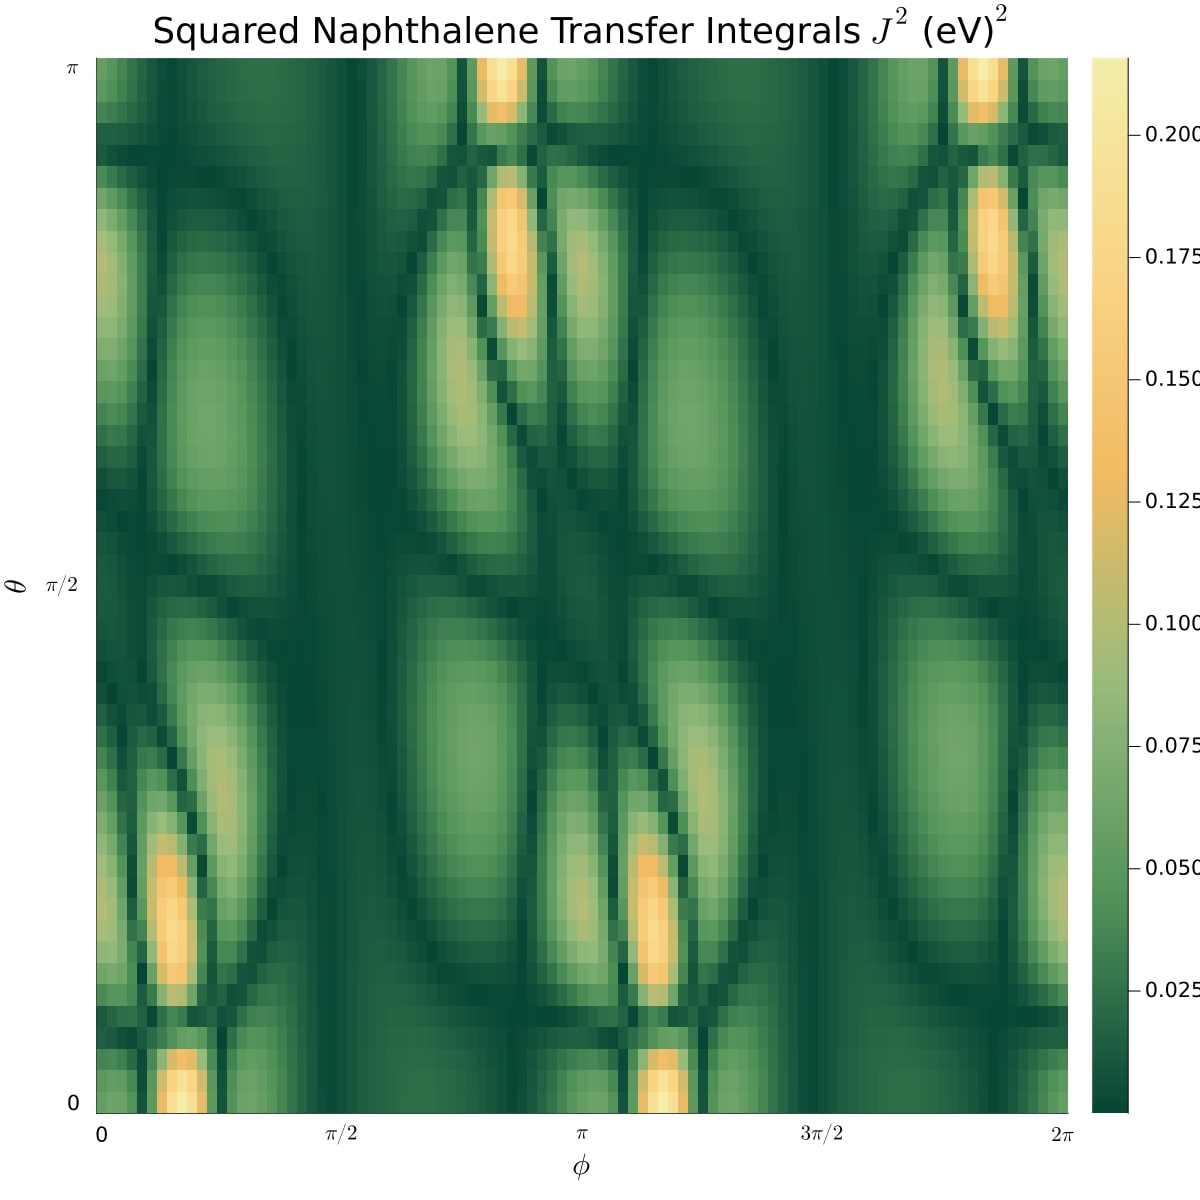
\includegraphics[width=1\linewidth,height=\textheight,keepaspectratio]{Figure/Chapter 4/1_Naphthalene/new_Naphthalene_J^2_heatmap.jpg}
  \caption{}
\end{subfigure}
\begin{subfigure}{.32\textwidth}
  \centering
  \includegraphics[width=1\linewidth,height=\textheight,keepaspectratio]{Figure/Chapter 4/1_Naphthalene/new_Naphthalene_logJ^2_heatmap.jpg}
  \caption{}
\end{subfigure}
\caption{
    \label{fig:4.3.1}
        (a), (b), and (c) show the heatmaps of the naphthalene dimer's transfer integral, the squared transfer integral , and the logarithm of the squared transfer integral.
}
\end{figure*}

\subsubsection{Representing Naphthalene Dimers}
\begin{figure*}[t]\centering
  \centering
  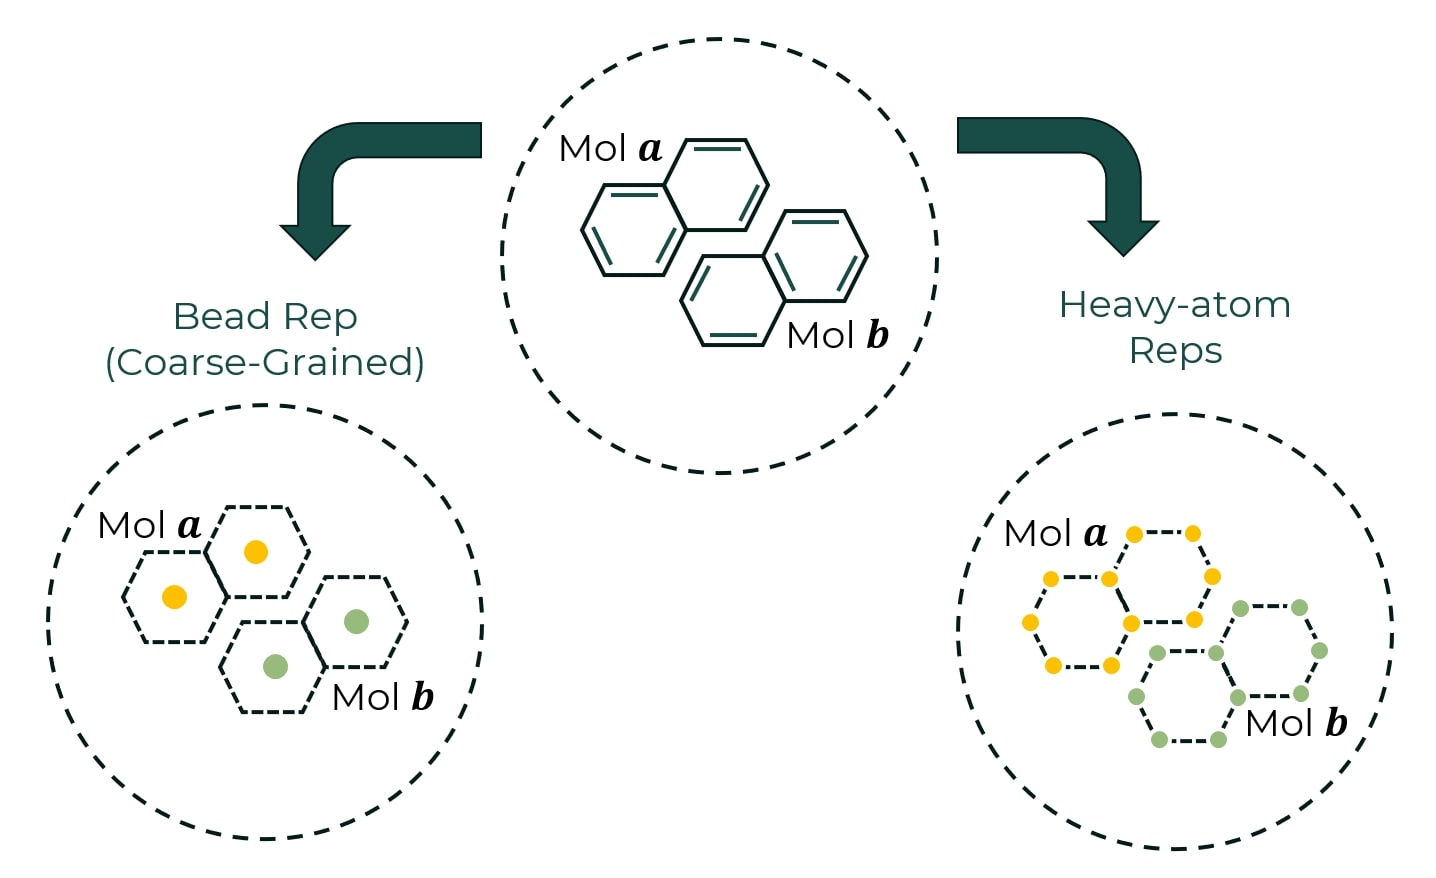
\includegraphics[width=1\linewidth,height=\textheight,keepaspectratio]{Figure/Chapter 4/1_Naphthalene/Representation1.jpg}
    \caption{
        \label{fig:4.4}
        Illustration of two types of molecular representations used for constructing ACE descriptors.
        %The central diagram shows a dimer of Naphthalene (Mol~$a$ and Mol~$b$). The left pathway depicts the \textit{Bead} (\textit{coarse-grained}) representation, in which each aromatic ring is represented by a single Bead. The right pathway illustrates the \textit{Heavy-atom} Representation, where only heavy (Heavy-atom) atoms are included. 
    }
\end{figure*}

Before constructing the ACE descriptors, we introduce an efficient representation of the naphthalene dimer aimed at reducing the dimensionality of the descriptor space while preserving key geometric and electronic features relevant to transfer integral prediction.

One such approach is the \textit{Bead} or \textit{Coarse-Grained Representation}, illustrated on the left pathway of Figure~\ref{fig:4.4}. This method is inspired by the recent work of Wang et al.~\cite{https://doi.org/10.48550/arxiv.2502.04661}, in which ACE models were successfully applied to coarse-grained molecular dynamics. We adapt this idea to model electronic coupling (transfer integrals) by constructing Bead ACE descriptors tailored to dimer interactions.

\begin{figure*}[t]\centering
  \centering
  \includegraphics[width=1\linewidth,height=\textheight,keepaspectratio]{Figure/Chapter 4/1_Naphthalene/RDF_Bead.jpg}
    \caption{
        \label{fig:4.5}
        Analysis of radial distribution functions (RDFs) and radial basis functions (RBFs) used in the ACE descriptor construction for the coarse-grained (Bead) representation. 
        %The top panel shows the intra- and intermolecular RDFs as a function of pairwise distance $r$, with a dashed line indicating the fixed centre-of-mass separation (12~\AA). The middle and bottom panels display the corresponding RBFs used to represent intra- and intermolecular environments, respectively. 
    }
\end{figure*}
Since the transfer integral is an intermolecular property, it is important to distinguish between atoms (or Beads) belonging to different molecules. As shown in Figure~\ref{fig:4.4}, we assign distinct element labels to each molecule: the yellow Beads in Mol~$a$ are treated as pseudo-\textbf{C} elements, while the green Beads in Mol~$b$ are labelled as pseudo-\textbf{Si} elements. This labelling enforces a separation of molecular environments and ensures that intra- and intermolecular interactions are treated distinctly within the ACE framework.

The next step is to analyse the intra- and intermolecular radial distribution functions (RDFs), plotted as a function of Bead-pairwise distance in the top panel of Figure~\ref{fig:4.5}.
The yellow histogram represents the intra-molecular RDF, while the red histogram shows the distribution of intermolecular pair distances. 
The dashed vertical line indicates the fixed centre-of-mass separation (12~\AA) used in our dimer configurations.

The analysis of the RDF guides the construction of radial basis functions (RBFs) using the \texttt{acemodel()} function, as illustrated in Figure~\ref{fig:4.6}. A discussion of the relevant hyperparameters is provided in Section~\ref{subsec:3.3.1}. 

\begin{figure*}[t]
  \centering
  \begin{lstlisting}[language=Julia]
model = (*@\textcolor{bEpic}{acemodel}@*)(elements = [(*@\textcolor{rEpic}{:C}@*),(*@\textcolor{rEpic}{:Si}@*),],
        order = 2,                 #3-body order
        totaldegree = 10,
        r0 = 12.0,                
        rcut = 13.6,
        pair_transform = ((*@\textcolor{rEpic}{:agnesi}@*), p = 19, q = 43),
        pair_envelope = ((*@\textcolor{rEpic}{:x}@*), 2, 2),
        Eref = [(*@\textcolor{rEpic}{:C}@*) => 0.0, (*@\textcolor{rEpic}{:Si}@*) => 0.0]
    )
  \end{lstlisting}
  \caption{\label{fig:4.6} Construction of a 3-body order ACE descriptor for a Bead structure using a total degree constraint of 10, an Agnesi radial transform, and a smooth polynomial envelope.}
\end{figure*}
%	@show length(model.basis)
%(*@\textcolor{bEpic}{> length(model.basis)}@*) = 338

Here, we emphasise the role of the envelope function used in constructing the RBFs. The default envelope \texttt{pair\_envelope = (:r, 2, 2)} leads to basis functions extending across both intra- and intermolecular regions (middle panel of Figure~\ref{fig:4.5}).
As shown in the bottom panel, modifying the envelope to \texttt{(:x, 2, 2)} localises the RBFs to the intermolecular range only.
In other words, RBFs are adapted to the relevant intermolecular RDF support ranges, enabling resolution where features are concentrated.
This ensures that the descriptor focuses on features relevant to transfer integrals, which are by nature intermolecular.

An additional hyperparameter, \texttt{Eref}, defines the one-body (atomic reference) energy.
By setting \texttt{Eref = 0} for each Bead type, we enforce the physical constraint that the transfer integral vanishes for isolated molecules or Beads.

\begin{figure*}[t]\centering
  \centering
  \includegraphics[width=1\linewidth,height=\textheight,keepaspectratio]{Figure/Chapter 4/1_Naphthalene/RDF_NH.jpg}
    \caption{
        \label{fig:4.7}
        Analysis of naphthalene dimer RDFs and RBFs used in the ACE descriptor construction for the Heavy-atom representation.
        %The upper panel shows the intra- and intermolecular RDFs as a function of pairwise distance , with a dashed line indicating the fixed centre-of-mass separation of 12~\AA.
        %The lower panel depicts the corresponding RBFs used to capture only intermolecular environments. 
    }
\end{figure*}
For the \textit{Heavy-atom Representation} shown on the right pathway in Figure~\ref{fig:4.4}, a similar analysis can be performed to construct the radial basis set for the corresponding ACE descriptors. 
In this representation, only heavy atoms (typically carbon) are included, thereby retaining chemically relevant geometric features while reducing the descriptor size.

The radial distribution functions (RDFs) for this representation are shown in the top panel of Figure~\ref{fig:4.7}, plotted as a function of pairwise distances between carbon atoms. 
As in the coarse-grained case, the yellow histogram corresponds to intramolecular RDFs, while the red histogram captures intermolecular distances. The fixed centre-of-mass separation is again marked by a dashed vertical line.

The choice of envelope functions for the radial basis can follow the same design as used in the Bead representation. 
Specifically, by applying an intermolecular envelope (e.g., \texttt{(:x, 2, 2)}), the radial basis functions can be restricted to the intermolecular distance range, thereby focusing the model on the features most relevant for predicting transfer integrals.

\subsubsection{ACEfit!}
\begin{figure*}[t]\centering
\begin{subfigure}{.5\textwidth}
  \centering
  
\includegraphics[width=1\linewidth,height=\textheight,keepaspectratio]{Figure/Chapter 4/1_Naphthalene/fitting_Bead_CSi_od2_td10_p19_q43_rcut136_N1350_mol.jpg}
  \caption{}
\end{subfigure}%
\begin{subfigure}{.5\textwidth}
  \centering
  
\includegraphics[width=1\linewidth,height=\textheight,keepaspectratio]{Figure/Chapter 4/1_Naphthalene/fitting_NH_CSi_od2_td10_p19_q43_rcut136_N1350_mol.jpg}
  \caption{}
\end{subfigure}
    \caption{
        \label{fig:4.8}
        The plots comparing predicted and reference energies for ACE models trained on 1350 structures out of a total of 4,753 dimer configurations. (a) Model trained using the \textit{Bead} representation. (b) Model trained using the \textit{Heavy-atom} representation. 
        %Yellow and green markers represent predictions on the full dataset and the training set, respectively.
    }
\end{figure*}
With all descriptors and hyperparameters defined, we now proceed to fit the ACE model to the transfer integral data of the naphthalene dimer. The reference transfer integrals were computed using the \textsc{PyMOO}, ZINDO-based method~\cite{Kirkpatrick2007}, package as implemented by J. M. Frost.

The ACE models constructed using the descriptors in Figure~\ref{fig:4.6} were trained on 1,350 dimer configurations out of a total of 4,753. The resulting fits using the \textit{Bead} and \textit{Heavy-atom} representations are shown in Figures~\ref{fig:4.8}a and~\ref{fig:4.8}b, respectively. Both models achieve high accuracy in predicting transfer integrals. The Bead-based model yields a root-mean-square error (RMSE) of 23.85~meV/molecule and a mean absolute error (MAE) of 16.86~meV/molecule. In comparison, the Heavy-atom model achieves even lower errors: RMSE = 13.63~meV/molecule and MAE = 9.84~meV/molecule.

These results are notable in that the predictive errors are of similar magnitude across the two representations, yet the computational cost of the Bead-based model is significantly lower—by approximately a factor of five. The Bead representation uses only four coarse-grained Beads per naphthalene dimer, while the Heavy-atom representation employs twenty carbon atoms per configuration. This efficiency gain results from the reduced number of sites per configuration.

Therefore, the Bead (or coarse-grained) representation may offer an advantage in high-throughput screening scenarios where computational efficiency is critical. On the other hand, when maximal predictive accuracy is required—for example, in detailed mechanistic studies or high-fidelity simulations—the Heavy-atom model provides superior performance.
\begin{figure*}[t]\centering
\begin{subfigure}{.45\textwidth}
  \centering
  \includegraphics[width=1\linewidth,height=\textheight,keepaspectratio]{Figure/Chapter 4/1_Naphthalene/Naphthalene_od_error.jpg}
  \caption{}
\end{subfigure}%
\begin{subfigure}{.45\textwidth}
  \centering
  \includegraphics[width=1\linewidth,height=\textheight,keepaspectratio]{Figure/Chapter 4/1_Naphthalene/Naphthalene_td_error.jpg}
  \caption{}
\end{subfigure}
    \caption{
        \label{fig:4.9}
        Hyperparameter sensitivity analysis of ACE models fitted to transfer integrals using Bead (solid) and Heavy-atom representations (dashed). 
        %(a) RMSE (solid) and MAE (dash-dot) as a function of interaction order ($\nu$), which controls the maximum $(\nu+1)$ body order of the ACE descriptor. (b) RMSE and MAE as a function of the total polynomial degree used in the basis.
    }
\end{figure*}

We also provide an analysis of hyperparameter fine-tuning with respect to the \texttt{order} (interaction order) and \texttt{totaldegree} parameters. Figure~\ref{fig:4.9} presents the performance of ACE models fitted to transfer integrals using Bead (solid lines) and Heavy-atom (dashed lines) representations. Additional fine-tuning on these two hyperparameters is provided in Appendix~\ref{sec:A.3.1} and \ref{sec:A.3.2}, respectively.

Panel (a) shows the root-mean-square error (RMSE) and mean absolute error (MAE) as a function of the interaction order $\nu$, which determines the maximum $(\nu + 1)$-body correlation captured in the ACE descriptor. As expected, increasing the interaction order improves accuracy for both representations, although with diminishing returns beyond $\nu = 4$.

Panel (b) illustrates the effect of increasing the total polynomial degree. Both representations benefit from increasing \texttt{totaldegree} up to a point of saturation (\texttt{totaldegree} $= 20$), after which performance plateaus or slightly worsens due to overfitting or numerical instability.

We can also see that this fine-tuning analysis supports the earlier discussion for Figure~\ref{fig:4.8}, confirming that the Heavy-atom representation consistently achieves lower errors than the Bead-based model across these two tested hyperparameter settings.

\begin{figure*}[t]\centering
\begin{subfigure}{.5\textwidth}
  \centering
  \includegraphics[width=1\linewidth,height=\textheight,keepaspectratio]{Figure/Chapter 4/2_Thiophene/od_basis.jpg}
  \caption{}
\end{subfigure}%
\begin{subfigure}{.5\textwidth}
  \centering
  \includegraphics[width=1\linewidth,height=\textheight,keepaspectratio]{Figure/Chapter 4/2_Thiophene/td_basis.jpg}
  \caption{}
\end{subfigure}
    \caption{
        \label{fig:4.10}
        Growth of ACE basis size as a function of key hyperparameters for 2- (solid) and 4- (dashdot) chemical species. %(a) Basis size also grows rapidly with the interaction order ($\nu$), reflecting the combinatorial increase in many-body terms. (b) Basis size increases exponentially with the total degree of polynomials.
    }
\end{figure*}
However, these improvements in accuracy come with an increased computational cost.
As shown in Figure~\ref{fig:4.10}, the size of the ACE basis set for 2-chemical species grows rapidly with both \texttt{order} and \texttt{totaldegree} values.
Higher values lead to a substantial increase in both memory usage and model training time.
These trends emphasise the compensation between model expressivity and computational efficiency in ACE model construction.

We also further analysed and fine-tunde additional hyperparameters, including cutoff radias \texttt{rcut}, parameters \texttt{p}, and \texttt{q} for controlling the envelop function of RBFs. 
The corresponding ACE fitting results and discussions, provided in Appendix~\ref{sec:A.3}, will justify the suitable range of these hyperparameters for bith Bead and Heavy-atom representation.


In the following sections, we apply the same analysis workflow to predict the transfer integrals of two additional molecular dimers: ethylene and thiophene. For these systems, the reference transfer integrals were generated using the \textsc{xtb-dipro} package~\cite{Kohn2023}, rather than \textsc{PyMOO}.
As discussed in Section~\ref{subsec:2.6.3}, \textsc{xtb-dipro} leverages a semi-empirical tight-binding framework, offering significantly lower computational costs compared to conventional density functional theory (DFT) methods. This makes it particularly well-suited for generating large datasets required for ACE model training.

\section{Ethylene and Thiophene Dimers} \label{sec:4.3}
\begin{figure*}[t]\centering
  \centering
  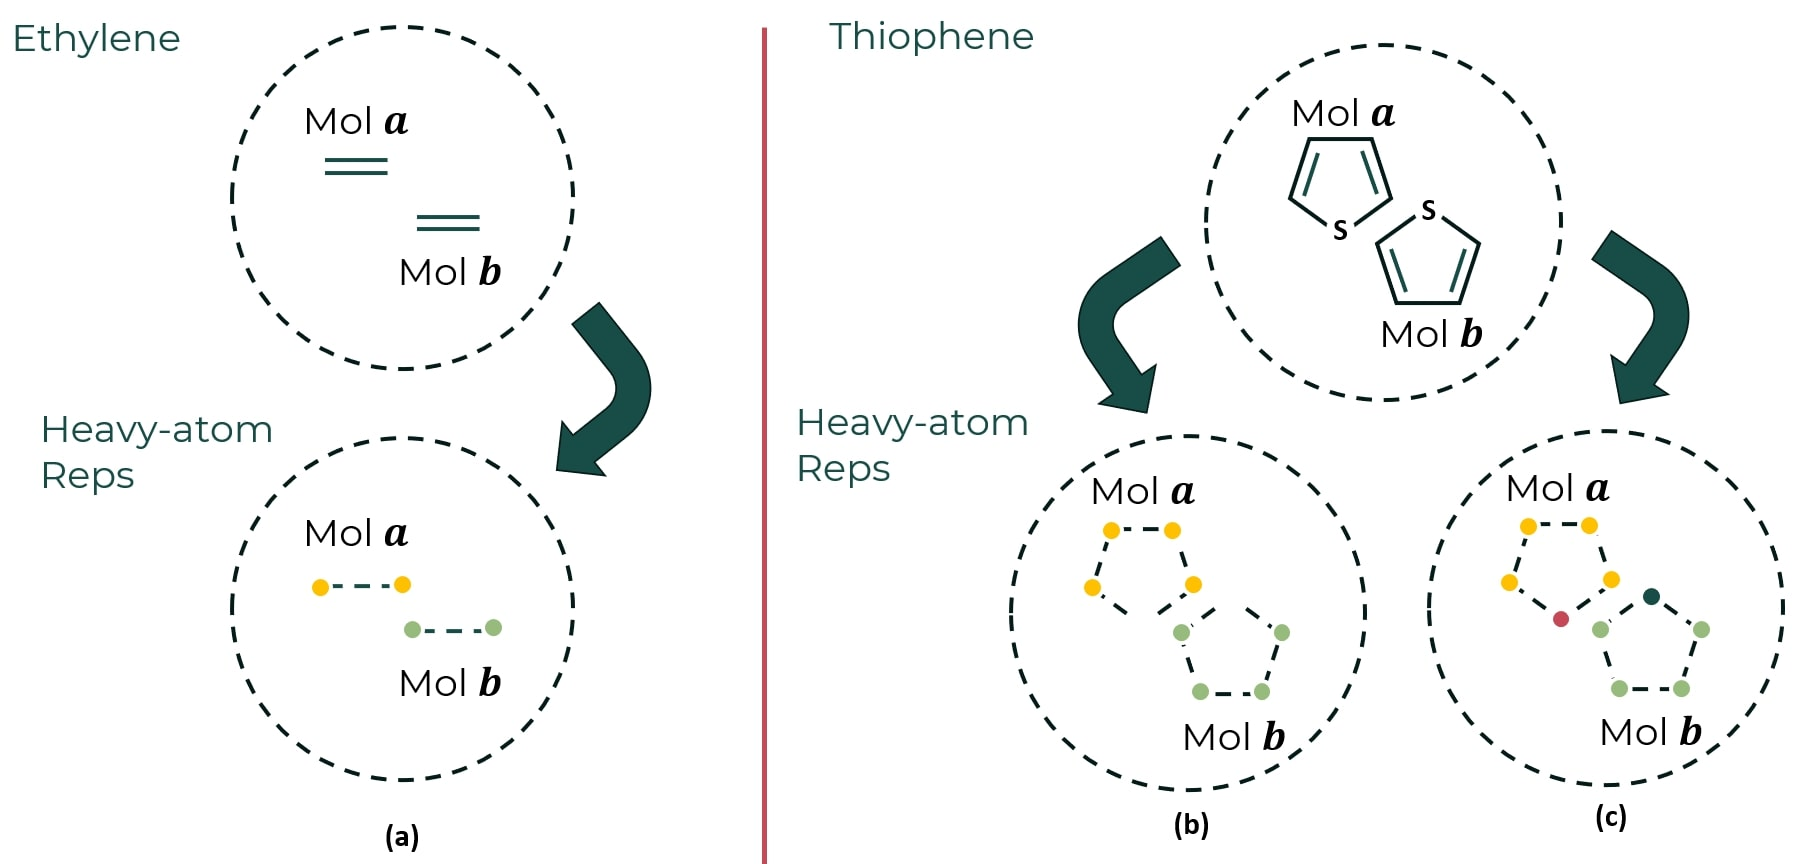
\includegraphics[width=1\linewidth,height=\textheight,keepaspectratio]{Figure/Chapter 4/3_Ethylene/Eth_Thi_repre.jpg}
    \caption{
        \label{fig:4.11}
        Illustration of three types of molecular representations used for constructing ACE descriptors for the ethylene and thiophene dimer (Mol~$a$ and Mol~$b$).
        %The central diagram shows the full molecular structures. Panel (a) depicts the \textit{Bead} (\textit{coarse-grained}) representation, in which each thiophene ring is represented by a single Bead. Panels (b) and (c) illustrate variations of the \textit{Heavy-atom} representation: (b) includes only carbon atoms, while (c) incorporates both carbon and sulphur atoms as distinct elements. 
    }
\end{figure*}

In this section, we examine suitable molecular representations for the ethylene and thiophene dimers and evaluate the corresponding ACE model predictions of their transfer integrals.

We, here, exclude the \textit{Bead} (coarse-grained) representation from consideration. For small molecules, this representation results in insufficient geometric resolution as a molecule turning into a point (psuedo-atom).
This makes it difficult to build effective radial basis sets and may lead to poor predictive performance.

We focus on the \textit{Heavy-atom} representation, as illustrated in Figure~\ref{fig:4.11}.  
On the left of the figure (a), the ethylene dimer is depicted using the standard Heavy-atom representation, incorporating only carbon atoms.  
On the right, we consider two variants for representing the thiophene dimer:  
pathway (b) includes only carbon atoms, while pathway (c) incorporates both carbon and sulphur atoms as distinct species.

\subsubsection{Analysis of Transfer Integral Surface and Training Sets}
\begin{figure*}[t]\centering
\begin{subfigure}{.32\textwidth}
  \centering
  \includegraphics[width=1\linewidth,height=\textheight,keepaspectratio]{Figure/Chapter 4/3_Ethylene/new_ethylene_J_surface.jpg}
  \caption{}
\end{subfigure}
\begin{subfigure}{.32\textwidth}
  \centering
  \includegraphics[width=1\linewidth,height=\textheight,keepaspectratio]{Figure/Chapter 4/3_Ethylene/new_ethylene_J^2_surface.jpg}
  \caption{}
\end{subfigure}
\begin{subfigure}{.32\textwidth}
  \centering
  \includegraphics[width=1\linewidth,height=\textheight,keepaspectratio]{Figure/Chapter 4/3_Ethylene/new_ethylene_logJ^2_surface.jpg}
  \caption{}
\end{subfigure}
\begin{subfigure}{.32\textwidth}
  \centering
  \includegraphics[width=1\linewidth,height=\textheight,keepaspectratio]{Figure/Chapter 4/3_Ethylene/new_ethylene_J_heatmap.jpg}
  \caption{}
\end{subfigure}
\begin{subfigure}{.32\textwidth}
  \centering
  \includegraphics[width=1\linewidth,height=\textheight,keepaspectratio]{Figure/Chapter 4/3_Ethylene/new_ethylene_J^2_heatmap.jpg}
  \caption{}
\end{subfigure}
\begin{subfigure}{.32\textwidth}
  \centering
  \includegraphics[width=1\linewidth,height=\textheight,keepaspectratio]{Figure/Chapter 4/3_Ethylene/new_ethylene_logJ^2_heatmap.jpg}
\caption{}
\end{subfigure}
\caption{
    \label{fig:4.12}
        (a), (b), and (c) show the heatmaps of the ethylene dimer's transfer integral, the squared transfer integral , and the logarithm of the squared transfer integral. (d), (e), and (f) illustrate the corresponding heatmap.
}
\end{figure*}

Figure~\ref{fig:4.12} and~\ref{fig:4.13} presents the transfer integral surfaces and heatmaps for the ethylene and thiophene dimers. Panels (a)–(f) correspond to the ethylene and thiophene dimer show the transfer integrals \( J \), their squared values \( J^2 \), and the logarithm of the squared values \( \log(J^2) \), respectively.
%Similarly, panels (d)–(f) display the same quantities for the 1,1-difluoroethylene dimer.
\begin{figure*}[t]\centering
\begin{subfigure}{.32\textwidth}
  \centering
  \includegraphics[width=1\linewidth,height=\textheight,keepaspectratio]{Figure/Chapter 4/2_Thiophene/new_Thiophene_J_surface.jpg}
  \caption{}
\end{subfigure}
\begin{subfigure}{.32\textwidth}
  \centering
  \includegraphics[width=1\linewidth,height=\textheight,keepaspectratio]{Figure/Chapter 4/2_Thiophene/new_Thiophene_J^2_surface.jpg}
  \caption{}
\end{subfigure}
\begin{subfigure}{.32\textwidth}
  \centering
  \includegraphics[width=1\linewidth,height=\textheight,keepaspectratio]{Figure/Chapter 4/2_Thiophene/new_Thiophene_logJ^2_surface.jpg}
  \caption{}
\end{subfigure}
\begin{subfigure}{.32\textwidth}
  \centering
  \includegraphics[width=1\linewidth,height=\textheight,keepaspectratio]{Figure/Chapter 4/2_Thiophene/new_Thiophene_J_heatmap.jpg}
  \caption{}
\end{subfigure}
\begin{subfigure}{.32\textwidth}
  \centering
  \includegraphics[width=1\linewidth,height=\textheight,keepaspectratio]{Figure/Chapter 4/2_Thiophene/new_Thiophene_J^2_heatmap.jpg}
  \caption{}
\end{subfigure}
\begin{subfigure}{.32\textwidth}
  \centering
  \includegraphics[width=1\linewidth,height=\textheight,keepaspectratio]{Figure/Chapter 4/2_Thiophene/new_Thiophene_logJ^2_heatmap.jpg}
\caption{}
\end{subfigure}
\caption{
    \label{fig:4.13}
        (a), (b), and (c) show the heatmaps of the thiophene dimer's transfer integral, the squared transfer integral , and the logarithm of the squared transfer integral. (d), (e), and (f) illustrate the corresponding heatmap.
}
\end{figure*}
These transfer integrals are generated by systematically rotating molecule~$b$ over the upper hemisphere around molecule~$a$, while maintaining a fixed centre-of-mass distance of 6.25~\AA for the ethylene dimer and of 7.50~\AA for the thiophene dimer.
The orientations are parameterised by the angular coordinates $\theta \in [0, \pi]$ and $\phi \in [0, 2\pi]$.

This visualisation helps to determine the most suitable target quantity for ACE model training. Despite some local skewness and discontinuities, the transfer integral surface $J$ appears noticeably smoother than those of $J^2$ and $\log(J^2)$, supporting its selection as a more appropriate target for regression with smooth basis function models such as ACE.

For gernerating the ethylene's training set, we sampled a three-dimensional surface,   
\[ J(x_{ab}, y_{ab}, z_{ab}) := J(r_{ab}, \theta_{ab}, \phi_{ab}),\] 
where the intermolecular separation \( r_{ab} \in [6.25,\; 7.00]~\text{\AA} \).
This separation range gauruntees the transfer integral results being smooth and continuous. 
The polar angle \( \theta_{ab} \in [0,\; \pi] \), while the azimuthal angle \( \phi_{ab} \in [0,\; 2\pi] \). The relative orientation of molecule \( B \) is fixed at \( \theta_{z} = \pi/6 \) with respect to molecule \( A \). This \(\theta_{z}\) will provide normal distributed radial distribution functions (RDFs) which are shown in next section. 

For the thiophene's training set, we use the same setting as the ethylene's one but change the intermolecular separation \( r_{ab} \in [7.25,\; 7.75]~\text{\AA}\).


\subsubsection{Representing Dimers}

\begin{figure*}[t]\centering
  \centering
  \includegraphics[width=1\linewidth,height=\textheight,keepaspectratio]{Figure/Chapter 4/3_Ethylene/RDF_ethylene.jpg}
    \caption{
        \label{fig:4.14}
        Ethylene dimer's RDFs and RBFs used in the ACE descriptor construction for the Heavy-atom representation.
        %The upper panel shows the intra- and intermolecular RDFs as a function of pairwise distance, with a dashed line indicating the fixed centre-of-mass separation of 6~\AA.
        %The lower panel depicts the corresponding RBFs used to capture only intermolecular environments. 
    }
\end{figure*}

We now proceed to construct the ACE descriptors for the ethylene and thiophene dimer, following the molecular representations illustrated in Figure~\ref{fig:4.11}. 

The left pathway (panel a) shows the Heavy-atom representation for the ethylene dimer. 
Similar to the naphthalene's case, to distinguish the two molecules, the atoms in Mol~$a$ is labelled as a pseudo-\textbf{C} element (yellow), while the atoms in Mol~$b$ is labelled as a pseudo-\textbf{Si} element (green).
This labelling enforces molecule-specific environments, allowing the ACE model to distinguish between intra- and intermolecular interactions.

\begin{figure*}[t]\centering
  \centering
  \includegraphics[width=1\linewidth,height=\textheight,keepaspectratio]{Figure/Chapter 4/2_Thiophene/RDF_thiophene_CSi_SO.jpg}
    \caption{
        \label{fig:4.15}
        Thiophene dimer RDFs and RBFs used in the ACE descriptor construction for the Heavy-atom representation.
        %The upper panel shows the intra- and intermolecular RDFs as a function of pairwise distance, with a dashed line indicating the fixed centre-of-mass separation of 6~\AA.
        %The lower panel depicts the corresponding RBFs used to capture only intermolecular environments. 
    }
\end{figure*}

The right pathway (panels b and c) illustrates two variations of the \textit{Heavy-atom} representation. Panel (b) includes only carbon atoms, while panel (c) includes both carbon and sulphur atoms. The sulphur atoms are assigned distinct element labels (e.g., red and dark green) to ensure that atomic species and molecular origin are treated separately. 

Again these representations enable a reduction in descriptor dimensionality while preserving essential geometric and electronic features relevant to transfer integral prediction. Moreover, the labelling strategy ensures clear separation of intra- and intermolecular contributions in the ACE basis.

As a next step, we analyse the radial distribution functions (RDFs) for intra- and intermolecular interactions. These are plotted as a function of pairwise distance between the atoms in the ethylene and thiophene dimer in the top panel of Figure~\ref{fig:4.14} and of Figure~\ref{fig:4.15}, respectively. The yellow histogram corresponds to intra-molecular RDFs, while the red histogram represents intermolecular RDFs. The dashed vertical line indicates the fixed centre-of-mass separation (6.5~\AA and 7.5~\AA) used in the ethylene and thiophene's dataset.
The both bottom panels illustrate the RBFs which can be extracted from the ACE model in the following discussion.

For the construction of the ACE model, we adopt the framework illustrated in Figure~\ref{fig:4.6}, applying it to the Heavy-atom representation containing only carbon atoms (Figure~\ref{fig:4.12}a and~\ref{fig:4.12}b). In each case, the parameters \texttt{r0} and \texttt{rcut} are appropriately adjusted to reflect the relevant intermolecular distance ranges observed in the thiophene dimer dataset.

Extending the model to the Heavy-atom representation that includes both carbon and sulphur atoms (Figure~\ref{fig:4.12}c) requires additional species which must be introduced to the ACE descriptor. In particular, sulphur atoms in molecules~$a$ and~$b$ are treated as distinct atomic types. For example, the species may be defined as in the code in Fig.~\ref{fig:4.16}.

\begin{figure*}[t]
  \centering
  \begin{lstlisting}[language=Julia]
model = (*@\textcolor{bEpic}{acemodel}@*)(elements = [(*@\textcolor{rEpic}{:C}@*),(*@\textcolor{rEpic}{:Si}@*),(*@\textcolor{rEpic}{:S}@*),(*@\textcolor{rEpic}{:O}@*),],
        ..., # c.f. Figure (*@\ref{fig:4.6}@*)
        Eref = [(*@\textcolor{rEpic}{:C}@*) => 0.0,(*@\textcolor{rEpic}{:Si}@*) => 0.0,(*@\textcolor{rEpic}{:S}@*) => 0.0,(*@\textcolor{rEpic}{:O}@*) => 0.0,]
    )
  \end{lstlisting}
  \caption{\label{fig:4.16} The extension of the construction of the ACE basis to support 4-chemical element structures.}
\end{figure*}
In this configuration, a pseudo-oxygen label (\texttt{:O}) is assigned to the sulphur atom in Mol~$b$ to ensure that the ACE model distinguishes between chemically identical atoms residing in different molecular environments. This strategy is consistent with the intermolecular nature of transfer integrals and enables explicit encoding of cross-molecular interactions in the basis construction.

\subsubsection{ACEfit!}
The fitting performance of the ACE models for the ethylene dimer is shown in Figure~\ref{fig:4.17}a. 
The model was trained on 2,000 structures out of a total of 8,000 and exhibit strong predictive performance, with the RMSEs (MAEs) of 3.20 (2.30)~$\mu$eV/molecule for the purely carbon (ethylene's Heavy-atom) representations.

\begin{figure*}[t]\centering
\begin{subfigure}{.33\textwidth}
  \centering
  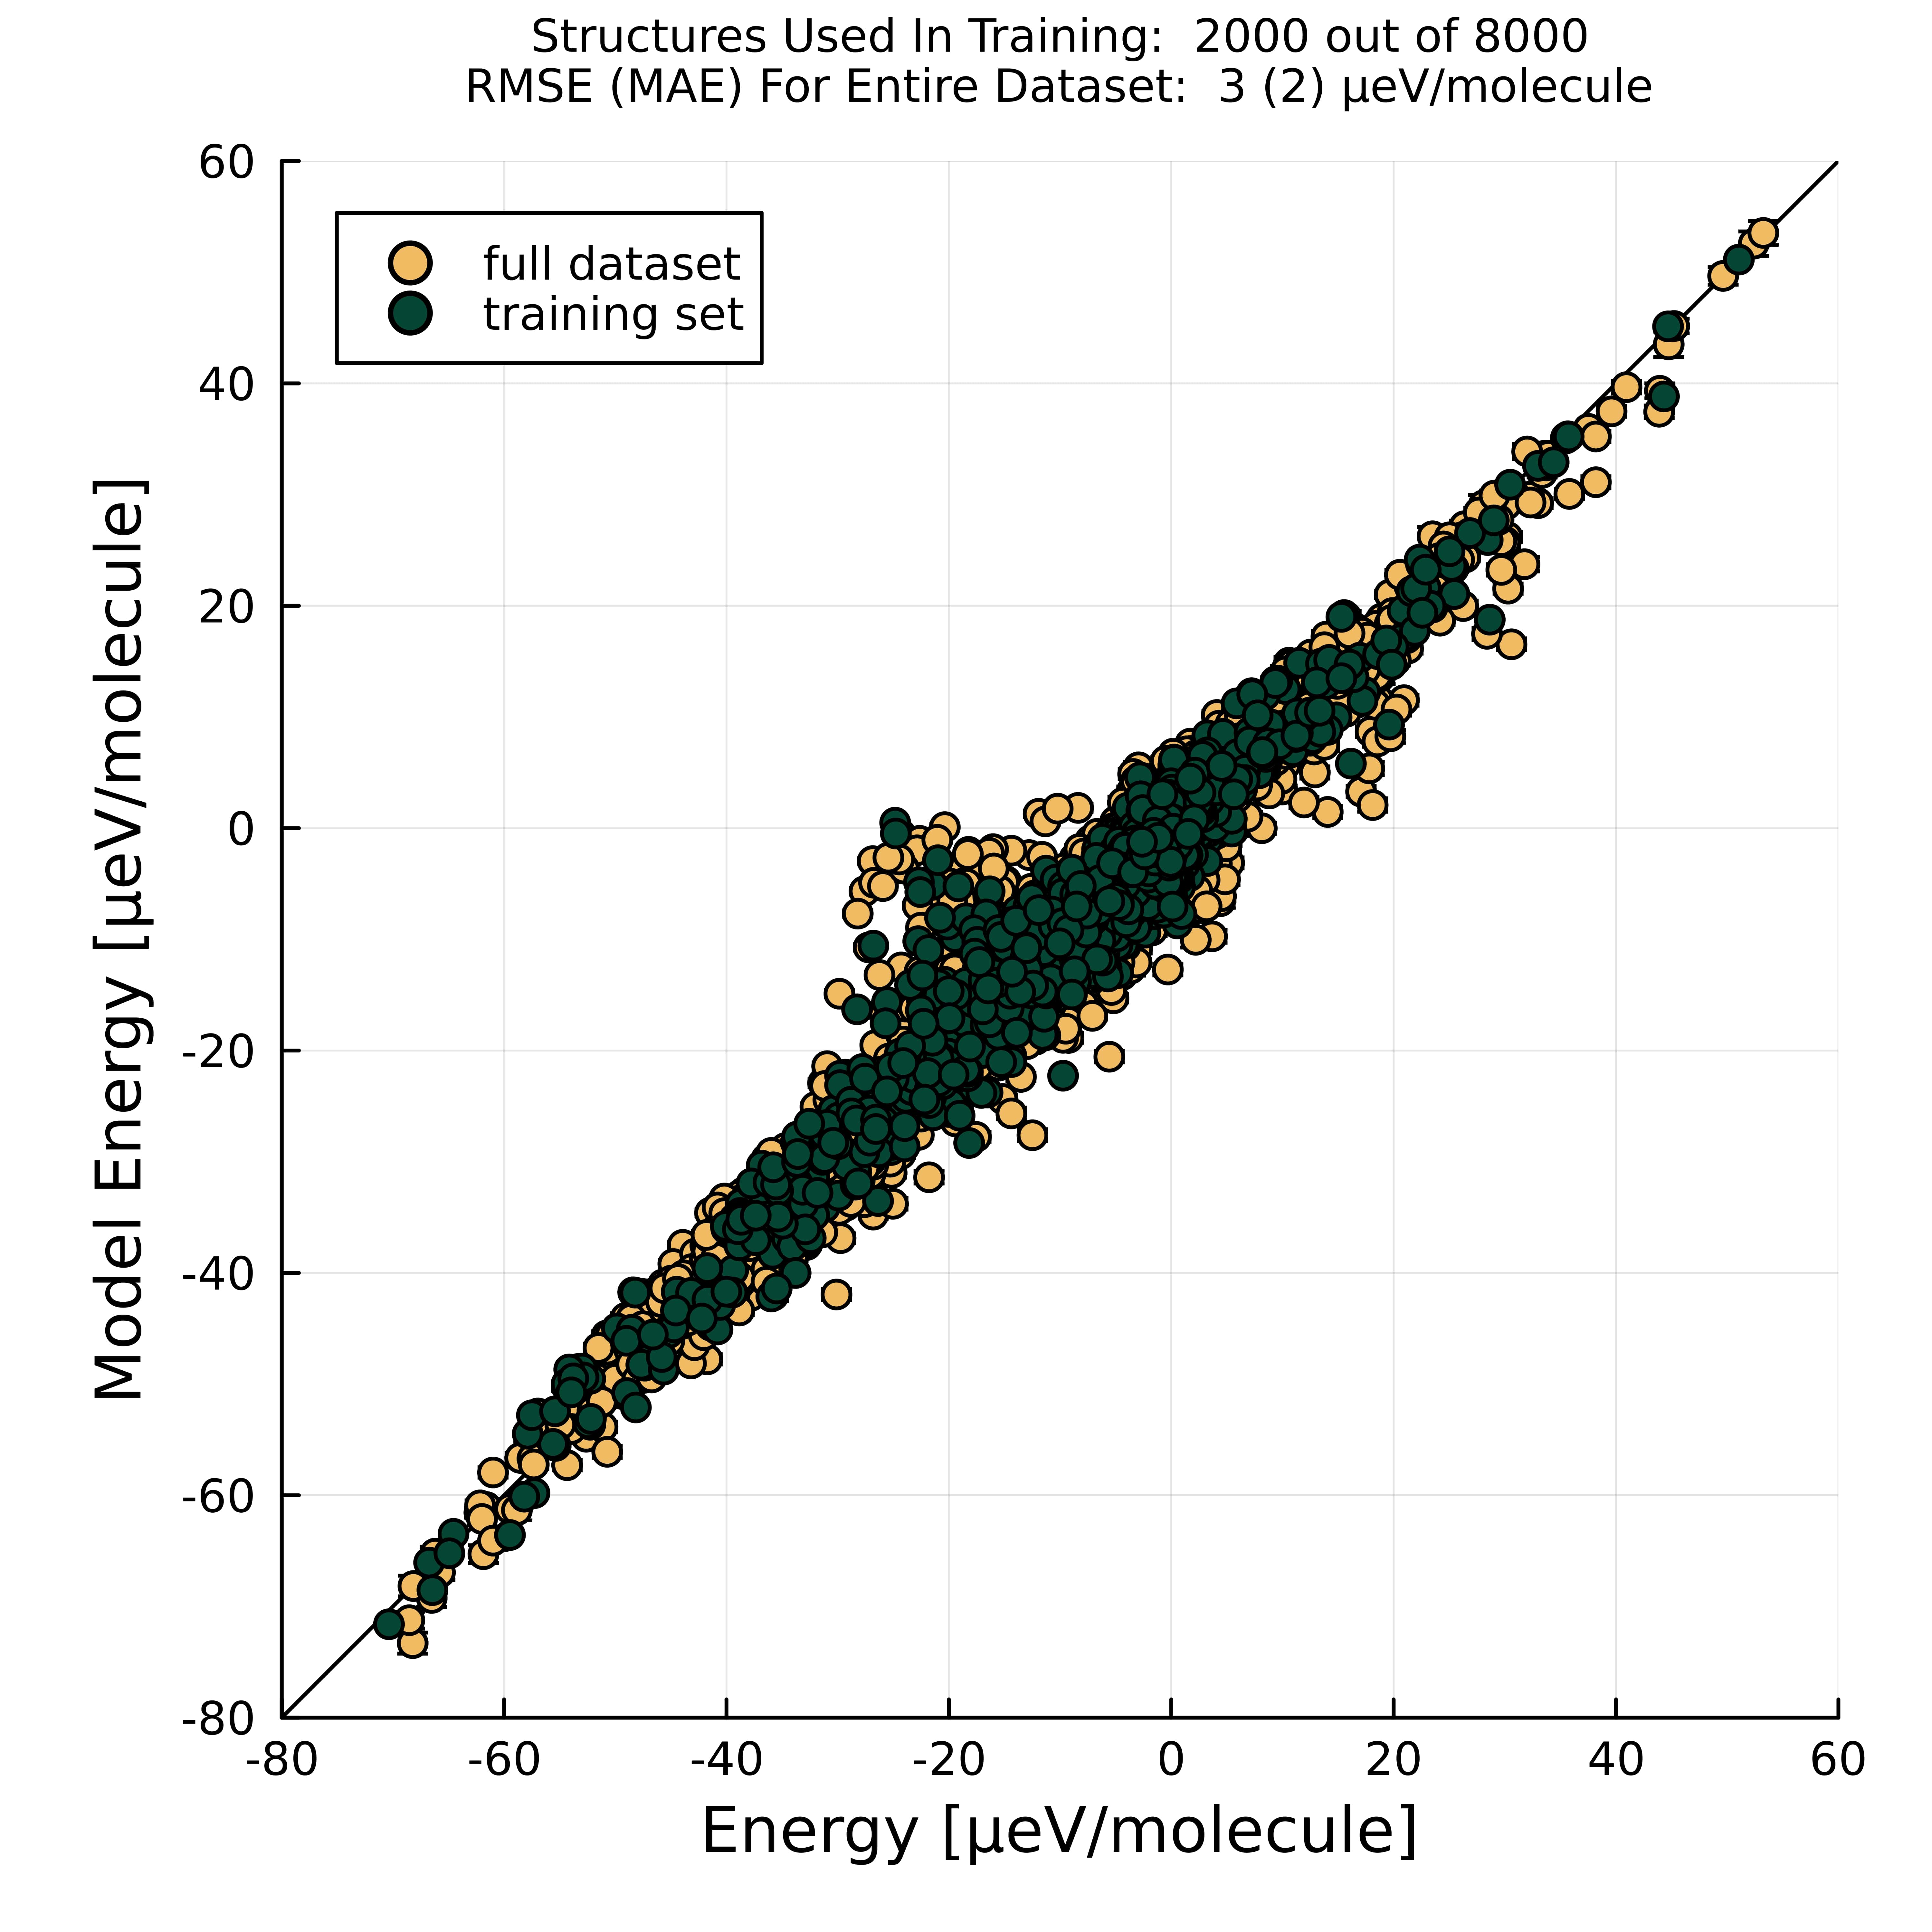
\includegraphics[width=1\linewidth,height=\textheight,keepaspectratio]{Figure/Chapter 4/3_Ethylene/fitting_NH_CSi_od2_td10_p19_q45_rcut7.5_N2000_rand_mol.jpg}
  \caption{Ethylene (HA-rep)}
\end{subfigure}%
\begin{subfigure}{.33\textwidth}
  \centering
  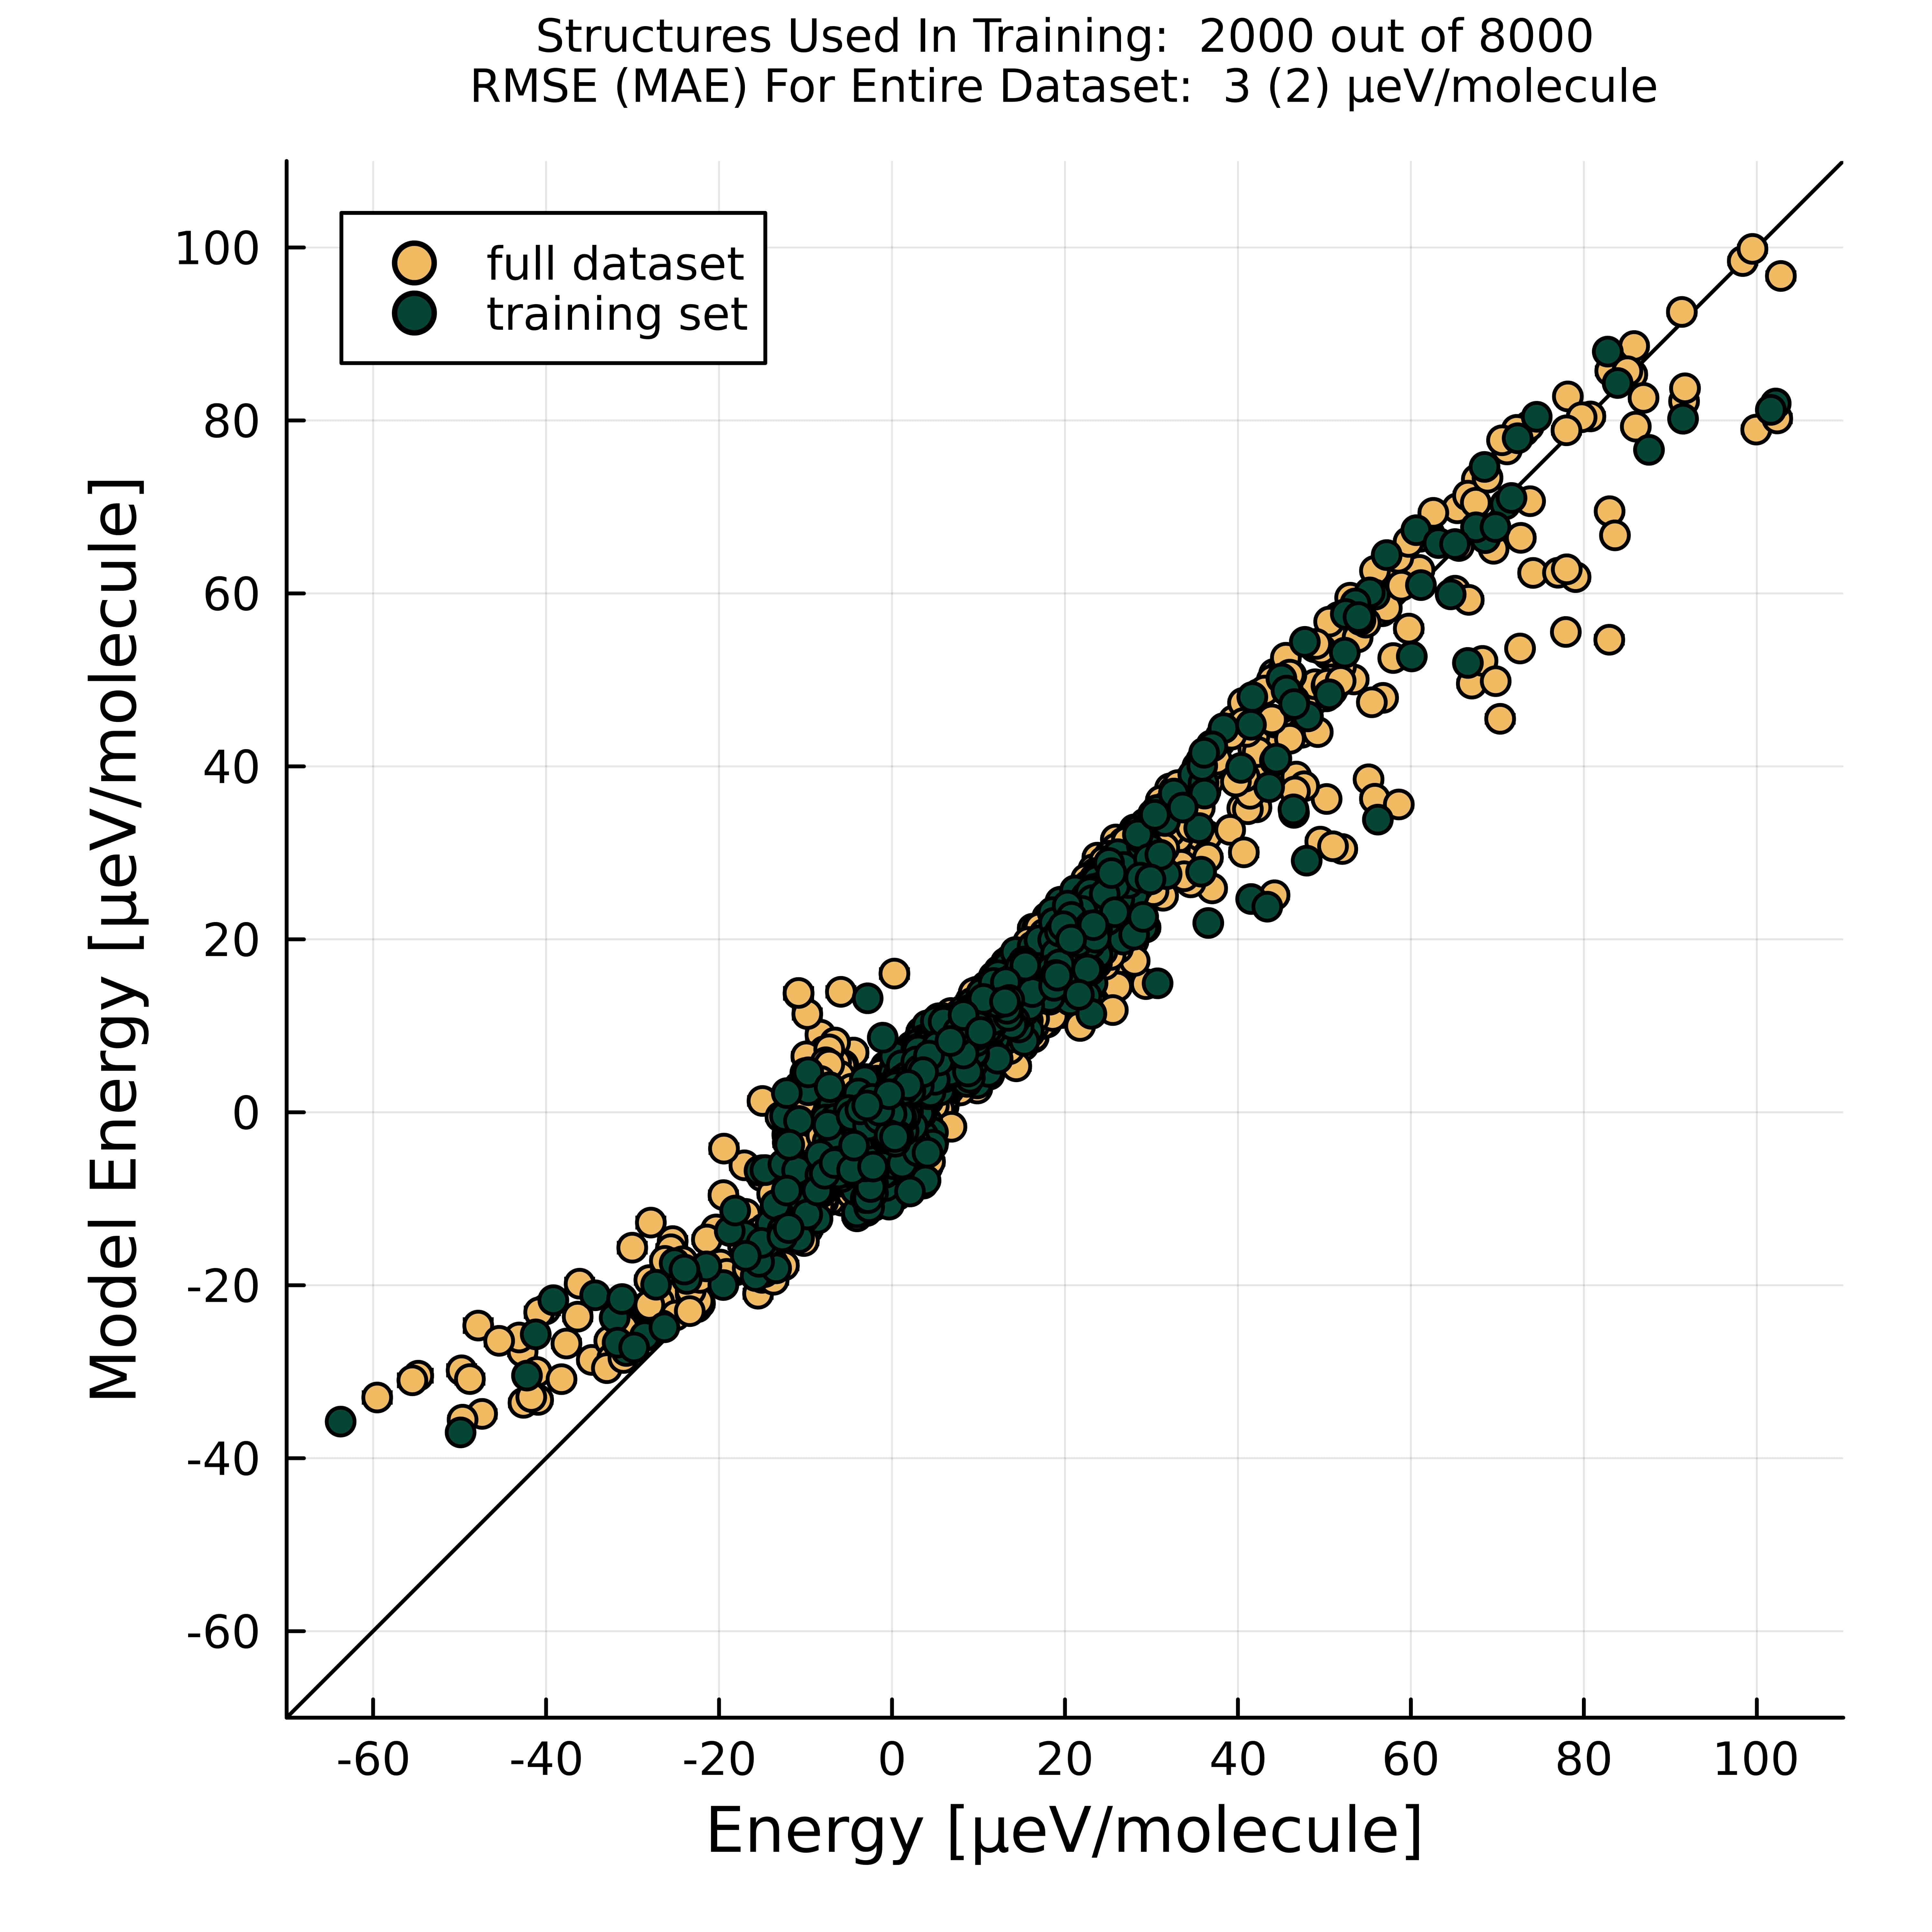
\includegraphics[width=1\linewidth,height=\textheight,keepaspectratio]{Figure/Chapter 4/2_Thiophene/fitting_NH_CSi_od2_td10_p19_q45_rcut9.0_N2000_rand_mol.jpg}
  \caption{Thiophene (HA-rep)}
\end{subfigure}
\begin{subfigure}{.33\textwidth}
  \centering
  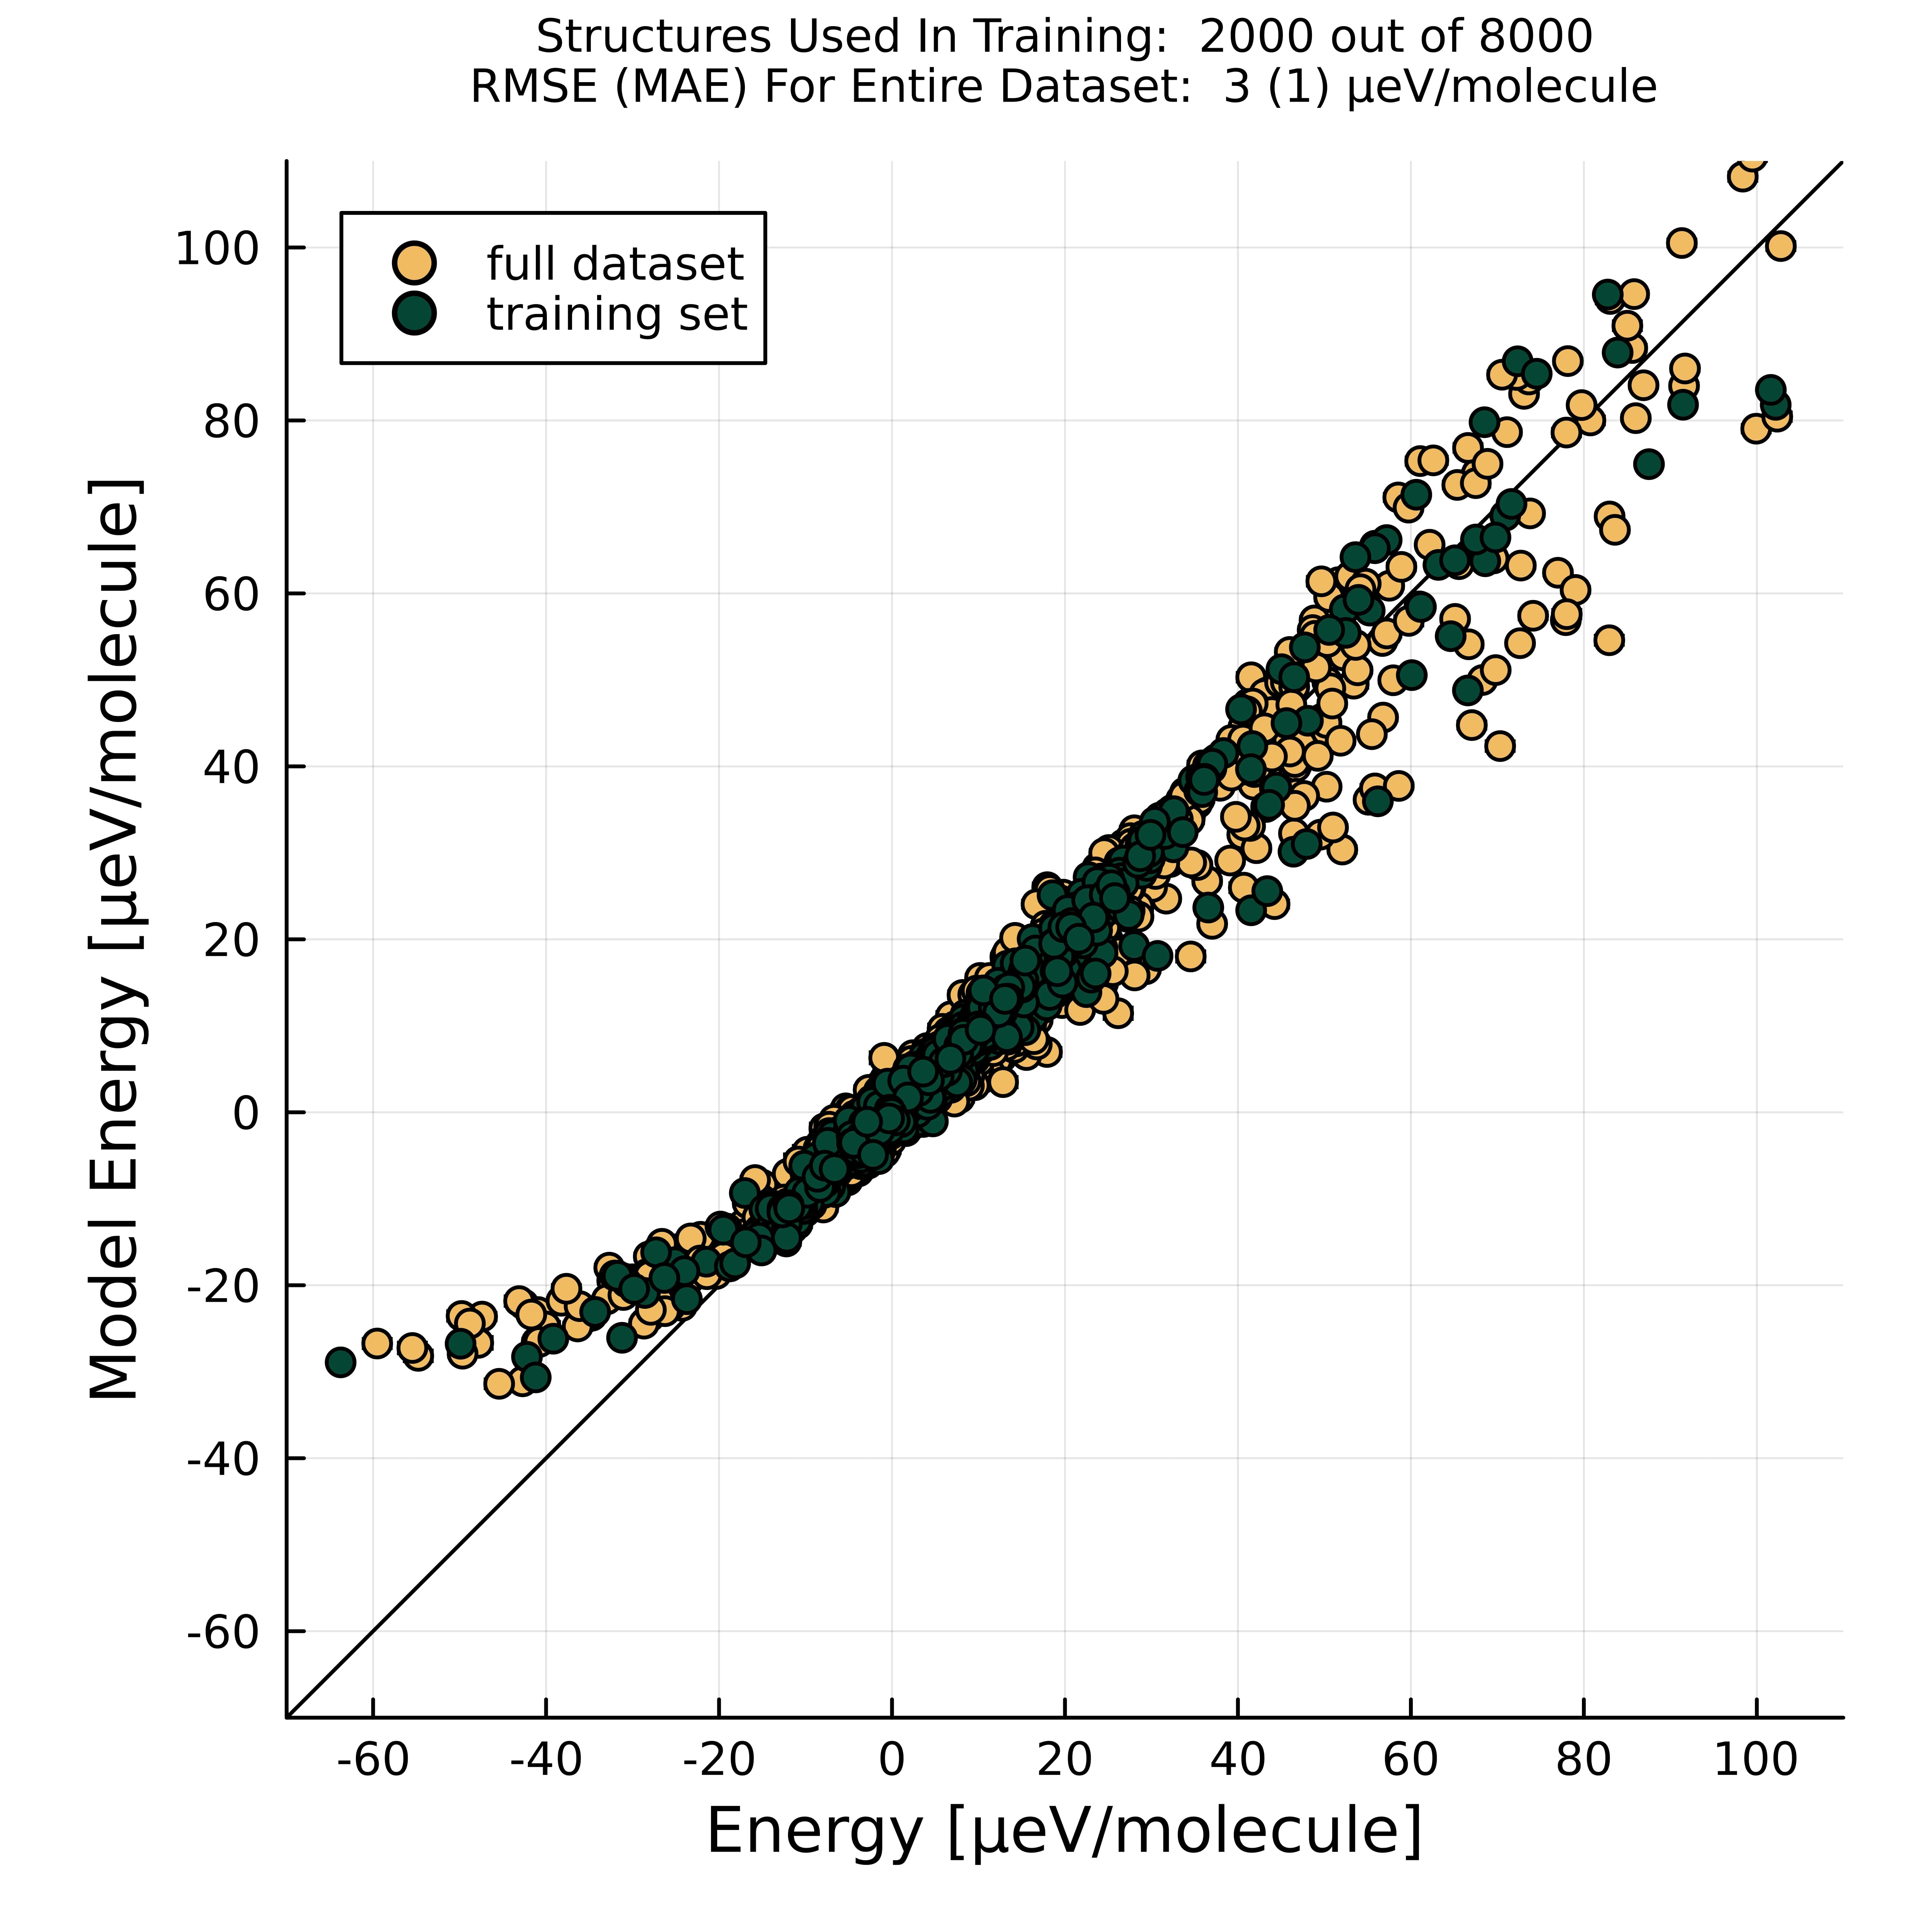
\includegraphics[width=1\linewidth,height=\textheight,keepaspectratio]{Figure/Chapter 4/2_Thiophene/fitting_NH_CSi_SO_od2_td10_p19_q45_rcut9.0_N2000_rand_mol.jpg}
  \caption{Thiophene (ext. HA-rep)}
\end{subfigure}
    \caption{
        \label{fig:4.17}
        The plots comparing predicted and reference transfer integrals for ACE models trained on 2,000 structures out of a total of 8,000 dimer configurations. 
        %(a) Model trained using the \textit{Heavy-atom} representation including only carbon atoms. (b) Model trained using the \textit{Heavy-atom} representation incorporating both carbon and sulphur atoms. Yellow and green markers represent predictions on the full dataset and the training set, respectively.
    }
\end{figure*}

The thiophene's fitting results are illustrated in Figures~\ref{fig:4.17}b and~\ref{fig:4.17}c.
Both of the results are fitted using the models were trained on 2,000 structures out of a total of 8,000 as the ethylene's case.
The fitting performance is also high with the RMSEs (MAEs) of 3.10 (2.03)~$\mu$eV/molecule for the purely carbon (thiophene's Heavy-atom) and of 2.65 (1.40)~$\mu$eV/molecule for the carbon-sulphur (thiophene's extended Heavy-atom) representations.

In comparing the two models, the incorporation of sulphur reduces the model error by around 15\% for the RMSE and approximately 40\% for the MAE, based on 2,000 training structures. 
This change, however, increases the computational cost associated with assessing the model descriptors (the basis set) and extends the duration required for fitting the ACE model: the training wall-clock time increases from 15 to 20 minutes (2,000 training structures).

\begin{figure*}[t]\centering
\begin{subfigure}{.45\textwidth}
  \centering
  \includegraphics[width=1\linewidth,height=\textheight,keepaspectratio]{Figure/Chapter 4/3_Ethylene/Ethene_od_error.jpg}
  \caption{}
\end{subfigure}%
\begin{subfigure}{.45\textwidth}
  \centering
  \includegraphics[width=1\linewidth,height=\textheight,keepaspectratio]{Figure/Chapter 4/3_Ethylene/Ethene_td_error.jpg}
  \caption{}
\end{subfigure}
    \caption{
        \label{fig:4.18}
        Hyperparameter sensitivity analysis of ACE models fitted to transfer integrals using Heavy-atom representations for fitting the ethylene's transfer integrals.
        %(a) RMSE (solid) and MAE (dash-dot) as a function of interaction order ($\nu$), which controls the maximum $(\nu+1)$ body order of the ACE descriptor. (b) RMSE and MAE as a function of the total polynomial degree used in the basis.
    }
\end{figure*}

Moreover, we perform a systematic hyperparameter study focusing on the \texttt{order} (interaction order) and \texttt{totaldegree} parameters. Figure~\ref{fig:4.18} illustrates the performance of ACE models trained to predict transfer integrals for the purely carbon (ethylene heavy-atom) representation.

Panel~(a) presents the RMSE and MAE as functions of the interaction order~$\nu$, which determines the maximum $(\nu+1)$-body correlations represented in the ACE descriptor. Increasing the interaction order improves model accuracy, with the optimal performance observed at $\nu = 3$. Panel~(b) shows the effect of the total polynomial degree, \texttt{totaldegree}, on fitting performance. Increasing \texttt{totaldegree} enhances accuracy up to a saturation point at \texttt{totaldegree}~$= 20$, beyond which the performance plateaus or slightly degrades due to overfitting and numerical instabilities.

The results for thiophene are presented in Figure~\ref{fig:4.19}. For the purely carbon (thiophene heavy-atom) representation, the trends are consistent with those observed for ethylene, while increasing the interaction order has little effect for the richer carbon–sulphur (extended heavy-atom) representation. In both cases, increasing the total polynomial degree improves accuracy, with optimal performance also achieved at \texttt{totaldegree}~$= 20$.

\begin{figure*}[t]\centering
\begin{subfigure}{.45\textwidth}
  \centering
  \includegraphics[width=1\linewidth,height=\textheight,keepaspectratio]{Figure/Chapter 4/2_Thiophene/Thiophene_od_error.jpg}
  \caption{}
\end{subfigure}%
\begin{subfigure}{.45\textwidth}
  \centering
  \includegraphics[width=1\linewidth,height=\textheight,keepaspectratio]{Figure/Chapter 4/2_Thiophene/Thiophene_td_error.jpg}
  \caption{}
\end{subfigure}
    \caption{
        \label{fig:4.19}
        Hyperparameter sensitivity analysis of ACE models fitted to transfer integrals using Heavy-atom representations (green) for fitting the ethylene's transfer integrals.
        %(a) RMSE (solid) and MAE (dash-dot) as a function of interaction order ($\nu$), which controls the maximum $(\nu+1)$ body order of the ACE descriptor. (b) RMSE and MAE as a function of the total polynomial degree used in the basis.
    }
\end{figure*}

We evaluated our model's efficiency across a variety of semiconducting substances. 
 The naphthalene model has an acceptable inaccuracy for charge-transfer simulations, with inaccuracies less than 2\% (9.84 meV/molecule).  
 The error for ethylene and thiophene is considerably elevated (5–10\%) when trained on 2,000 samples, suggesting a necessity for enhanced inductive biases for these systems. 
 We propose that this decreased performance results from the model's capacity to deduce the orientation in the case of ethylene (heavy atoms) and the distinct chemistry of the $C_2$ and $C_3$ carbons in thiophene, which we drive the model to combine. 
 There is substantial valuable work to be carried out experimenting with the fitting of complicated organic electronic molecules of contemporary technical significance, as well as with other structural representations. 

To contextualise our findings, we compare them to existing literature. 
 This comparison is constrained by the use of different datasets. 
 The establishment of standard standards for organic electronic transfer integrals will greatly assist the community in the development and validation of these methodologies, rendering them efficient tools for modelling real materials. 

We emphasise the data efficiency of our approach. 
 Recent studies\cite{Lin2023,Wang2020} reveal mean absolute errors (MAEs) of 1.99 meV for naphthalene and 0.27 meV for ethylene using multi-stage kernel ridge regression (KRR) models with 15,000 to 40,000 training samples \cite{Lin2023,Wang2020}, and approximately 6.5 meV for naphthalene utilising artificial neural networks (ANNs) trained on 120,000 samples \cite{Wang2020}. Our naphthalene model achieves comparable accuracy with 1,350 samples.
 
\section{Conclusions and Future Work} \label{sec:4.4}
In this chapter, we introduced an ACE-based method that uses physically motivated representations to predict transfer integrals (electronic couplings) in organic molecular dimers. Two different schemes were presented and assessed for various classes of molecular dimers: the \textit{Bead} (or \textit{Coarse-Grained}) representation and the \textit{Heavy-atom} representation. In order to balance computational efficiency and ACE descriptor resolution, these representations were created to capture important geometric and electronic features related to intermolecular charge transport.

Our findings indicate that the \textit{Heavy-atom} representation consistently outperforms the \textit{Bead} representation in terms of prediction accuracy, particularly for small or chemically heterogeneous systems such as thiophene and 1,1-difluoroethylene. In comparison with larger, more symmetric dimers like naphthalene, both representations produce satisfactory results, even though the Bead-based model offers significant computational advantages due to its reduced dimensionality. However, for smaller dimers such as ethylene, the Bead representation fails entirely, yielding trivial predictions due to insufficient configurational resolution. Across all systems, we observed that the transfer integral surfaces often exhibit discontinuities and sharp features that are challenging to learn using smooth basis sets such as those in ACE. Highly localised radial distribution functions (RDFs) make this problem more severe by reducing the radial basis functions' effective support.

Although increasing the model complexity—by raising the interaction \texttt{order} and \texttt{totaldegree} parameters—leads to a larger basis set, this does not always result in improved predictive performance. The mismatch between the peaked data distributions and the smooth ACE basis leads to inefficiencies and, in some cases, diminishing returns. Consequently, further improvements must come from better alignment between descriptor resolution and the data characteristics.

For future works, there are several promising directions for future work. First, generating training datasets with varied centre-of-mass separations may enhance the radial sampling, thus improving descriptor coverage and reducing interpolation errors. Second, transforming the target quantity—for example, fitting to $\log(J^2)$ instead of $J$ or $J^2$—may improve learning outcomes by producing smoother and more Gaussian-like distributions. Third, integrating ACE descriptors into hybrid architectures such as graph neural networks or message-passing schemes \cite{https://doi.org/10.48550/arxiv.2206.07697, Batatia2025} could offer improved representation of anisotropic and long-range interactions. Additionally, representation learning approaches that optimise atom-type embeddings or construct chemically informed basis functions may improve performance in systems with strong electronic heterogeneity. Finally, applying these ACE-based models to larger-scale simulations of charge transport in organic materials would allow us to assess their utility in realistic device-level scenarios.

To wrap up, this study shows that ACE is a capable and versatile tool for building surrogate models of transfer integrals. The approaches explored here form a solid starting point for further work on machine-learning-based models of charge transport in organic materials. That said, there are still clear challenges—especially for systems that are small, lack symmetry, or involve chemically diverse atoms—where the model struggles to capture all the relevant details.

This chapter has designed and extensively assessed an Atomic Cluster Expansion (ACE) framework for predicting electronic transfer integrals in organic molecular dimers. By expressing \( J_{ab} \) as a summation of localised, symmetry-conserving site contributions, the proposed methodology guarantees Hermitian symmetry, rotational and translational invariance, and spatial locality—attributes that are crucial for accurately depicting intermolecular electronic couplings in a physically relevant context.

 Two molecular representations were presented: a coarse-grained \textit{Bead} representation and a chemically informed \textit{Heavy-atom} representation.  The Bead method delivers notable computational performance, especially for extensive aromatic systems, whilst the Heavy-atom representation ensures enhanced accuracy by preserving critical geometric and chemical information.  ACE models demonstrated high predictive accuracy across naphthalene, ethylene, and thiophene dimers with relatively limited training datasets, showcasing superior data efficiency compared to traditional kernel- and neural-network-based methods.

 An hyperparameter investigation indicated that model performance enhances with rising interaction order and polynomial degree until a saturation threshold is reached, after which further complexity results in decreasing returns or causes numerical instability.  In chemically simple systems like ethylene, increased interaction orders significantly improve accuracy; yet, in more heterogeneous systems such as thiophene with an extensive carbon-sulphur representation, the advantage becomes negligible due to the existing chemical variety enriching the descriptor.  The ideal polynomial degree was consistently identified at \texttt{totaldegree} \(= 20\).

The comparative investigation of various molecular representations and hyperparameter configurations demonstrates that ACE is highly effective at capturing the geometric dependency of transfer integrals, even in chemically diverse systems. The study simultaneously identifies specific limitations: in systems where electronic coupling fluctuates substantially with geometry or displays significant anisotropy, the continuous polynomial framework of the ACE basis might require larger basis sets or more focused sampling of configuration space to attain equivalent accuracy. These observations point toward promising directions for future development, including hybrid descriptor schemes, improved target transformations (such as modelling $\log J^{2}$ to stabilise learning), and tighter integration with graph-based neural descriptors or message-passing schemes \cite{https://doi.org/10.48550/arxiv.2206.07697, Batatia2025}.

This chapter's results indicate that ACE offers a robust, symmetry-preserving, and computationally scalable framework for simulating intermolecular electrical interactions.  The technique provides reliable predictions while maintaining sufficient flexibility to address the complicated nature of real molecular materials.  This offers a robust basis for future extensive charge-transport simulations in organic semiconductors and provides an opportunity to expand ACE-based models to more sophisticated chemical and structural contexts.
